\documentclass{mnitjaipur}
\usepackage{placeins}
\usepackage{longtable}
\usepackage{float}
\usepackage{listings}
\usepackage{xcolor}
\usepackage{tikz}
\usepackage{url}
\usetikzlibrary{arrows.meta,positioning,shapes.geometric}

\documenttype{2}
%%% 1 : minor project report
%%% 2 : major project report

\department{Computer Science \& Engineering}
\stream{0}
\degree{2}

\areaResearch{eBPF for Android Kernel Monitoring}
\heading{Aether: A Suite of eBPF based tools for Real time Android Kernel Monitoring}
\groupcount{2}

\nameI{Shubham Singh}
\rollI{2022UCP1949}
\genderI{Male}

\nameII{Aakash Runthala}
\rollII{2022UCP1267}
\genderII{male}

\batchmonth{July}
\batchyear{2023}
\qualification{B.Tech.}

\logo{MNITlogo}

\thisdate{14}
\thismonth{May}
\thisyear{2026}

\supervisor{Prof. Vijay Laxmi}
\supervisordept{Computer Science \& Engineering}
\supervisorcollege{Malaviya National Institute of Technology Jaipur}
\supervisorcollegeloc{JLN Marg, Jaipur, Rajasthan 302017, INDIA}
\cosupervisor{}
\cosupervisorAffliation{Affiliation}

\keys{~\textit{eBPF};~\textit{Android kernel};~\textit{observability};~\textit{security monitoring};~\textit{network stack}}

\ack{
I would like to express my sincere gratitude to Dr. Vijay Laxmi for her guidance, feedback, and encouragement throughout this project. I also thank the Department of Computer Science and Engineering, MNIT Jaipur, for providing the laboratory facilities and learning environment. I am grateful to my peers and friends for their discussions and support during development and testing.
}

% Listings setup
\definecolor{codebg}{rgb}{0.97,0.97,0.97}
\definecolor{codeframe}{rgb}{0.85,0.85,0.85}
\lstset{
  basicstyle=\ttfamily\small,
  backgroundcolor=\color{codebg},
  frame=single,
  rulecolor=\color{codeframe},
  breaklines=true,
  showstringspaces=false,
  tabsize=2,
  captionpos=b
}

\begin{document}

\frontpage
\certificate
\acknowledgment
\declaration
\setstretch{1.5}
\setlength{\parindent}{0pt}

\begin{abstract}
\noindent This project delivers a suite of five eBPF-based utilities for Android kernel observability, focusing on process lifecycle, execution behavior, privilege transitions, file activity, and packet tracing. The motivation is the lack of lightweight, Android-oriented tools that expose kernel-level behavior without heavy instrumentation. We implement targeted kernel hooks using tracepoints, kprobes, and TC ingress programs, and stream structured events to user space via ring buffers. The tools are designed to be verifier-friendly and provide low-noise signals for security analysis and system debugging.

We validate the tools on a physical Android device (Motorola G96 5G, SoC Qualcomm SM7450 Snapdragon 695, Architecture AArch64 ARM 64-bit, Kernel Version 5.10.233-android12-9, Kernel Compiler Android Clang 12.0.5) and demonstrate that each tool produces actionable output with minimal overhead. The results show that the suite can detect suspicious execution patterns, privilege escalations, file modifications, and network activity in a unified workflow. These findings establish a practical, extensible foundation for Android kernel monitoring and security analytics.

Each tool in the suite is implemented as a standalone binary that can be deployed independently, enabling targeted monitoring without loading unnecessary kernel hooks. The ring buffer transport mechanism ensures bounded memory usage and predictable event delivery latency, even under high-throughput workloads. All tools are compiled using CO-RE (Compile Once, Run Everywhere) techniques, allowing the same binary to adapt to different kernel struct layouts at load time without recompilation. This design makes the suite suitable not only for research and debugging but also as a lightweight foundation for production-grade Android security telemetry pipelines.
\end{abstract}

\roleauthor
\addcontentpages
\pagenumbering{arabic}

\clearpage
\chapter{Introduction}
Android has established itself as the world’s most dominant mobile operating system, powering billions of devices and handling sensitive personal and enterprise data. This ubiquity, combined with its open-source nature, makes it a prime target for sophisticated malware and zero-day exploits \cite{smalley2013security, gki2023aosp}. While the Android stack incorporates robust security layers—such as SELinux, seccomp filters, and application sandboxing—these mechanisms often operate as "black boxes" from an observability standpoint \cite{aron2015android, ebpfio2024, lindorfer2023monitoring}. Conventional monitoring techniques, like ptrace-based tracing or heavy audit logging, often introduce unacceptable performance overhead or require intrusive kernel modifications that are impractical for production environments.

The necessity for real-time, low-overhead intrusion detection has never been greater. Current threats leverage short-lived processes and rapid privilege escalations to evade static analysis and traditional sandboxes. To address this, we present a suite of eBPF-based utilities designed for high-fidelity, in-kernel telemetry. By hooking directly into tracepoints and kprobes, these tools provide actionable signals regarding process lifecycles, credential transitions, and network ingress with minimal system impact. This approach bridges the gap between stringent security enforcement and the need for transparent, real-time behavioral observability in modern mobile ecosystems\cite{ebpf_linux_doc,libbpf_doc}.

\section{Background}
The Android ecosystem is characterized by extreme device diversity, spanning a vast range of hardware configurations, kernel versions, and vendor-specific modifications. This fragmentation creates a significant challenge for security monitoring, as traditional kernel-module-based solutions often require recompilation for every specific device target. The introduction of the Generic Kernel Image (GKI) in recent Android versions has mitigated some of these issues, providing a more stable base for technologies like eBPF \cite{gki2023aosp}. Extended Berkeley Packet Filter (eBPF) allows for the safe execution of bytecode within the kernel without altering the source code, making it an ideal candidate for cross-device monitoring \cite{ebpfio2024}.

However, the shift toward deep kernel monitoring raises critical privacy concerns. Because kernel-level hooks can observe all system calls and data flows, there is a risk of inadvertently capturing sensitive user information. Effective monitoring tools must therefore balance "observability" with "privacy-by-design," focusing on metadata and structural event patterns rather than raw data payloads. This background sets the stage for a real time monitoring suite that is portable across the Android landscape while remaining sensitive to the performance and privacy constraints of mobile users.


\section{Motivation}
Security incidents on mobile devices often involve short-lived processes, rapid privilege changes, or hidden file and network activity. A lightweight observability suite that runs close to the kernel can highlight these behaviors in real time. Most existing tools in the Linux ecosystem assume desktop-style environments or require heavy tracing stacks, making them less suitable for Android-specific workflows.

Typical scenarios that benefit from these signals include:
\begin{itemize}
  \item Detecting abnormal shell invocation sequences after an app is compromised.
  \item Identifying privilege escalations by observing credential changes.
  \item Tracing file modifications in sensitive paths.
  \item Inspecting inbound packets at the earliest possible point in the stack.
\end{itemize}

\section{Problem Statement}
The core problem addressed is the lack of lightweight, Android-oriented real time kernel observability tools that provide actionable signals without requiring invasive kernel changes. The goal is to design and implement a verifier-friendly eBPF suite that is compatible with Android kernels, produces concise outputs, and supports multi-stage attack analysis.

\section{Objectives}
The objectives of the study are as follows:
\begin{itemize}
    \item To design and implement a kernel-level observability framework using eBPF for monitoring inter- and intra-process as well as application-level communication on Android devices.
    \item To observe and analyze low-level system activities, including process execution, memory utilization, and filesystem access.
    \item To assess the usefulness of kernel-level observability in identifying monitoring limitations and potential security vulnerabilities.
\end{itemize}


% \section{Scope and Limitations}
% The scope of this project is kernel-level observability for Android using eBPF programs attached to tracepoints, kprobes, and TC ingress. The suite focuses on read-only telemetry rather than active enforcement. The following are outside the current scope:
% \begin{itemize}
%   \item Egress network tracing and full packet capture.
%   \item User-space instrumentation (library call tracing or app internals).
%   \item Kernel module based monitoring or LSM-based enforcement.
%   \item Deep application context such as package name mapping or Java stack traces.
% \end{itemize}

\section{Contributions}
The key contributions of this work are:
\begin{itemize}
  \item A five-tool eBPF suite for Android kernel observability.
  \item Consistent, low-overhead data collection using BPF ring buffers. A ring buffer (also called a circular buffer) is a fixed-size, contiguous memory region in which a write pointer advances in a wrap-around fashion; it differs from a classic queue in that it is lock-free, operates in shared kernel--user memory without copy overhead, and discards the oldest data rather than blocking when full. The BPF ring buffer (\texttt{BPF\_MAP\_TYPE\_RINGBUF}) adds producer-side reservation semantics so that an eBPF program can atomically reserve a slot, fill it in place, and submit it in a single pass, avoiding the per-CPU allocation required by the older perf event array.
  \item Android-aware heuristics and namespace-aware event output. eBPF fully supports namespace-aware observability on Android: each event record includes the process namespace inode (\texttt{inum}), allowing events from isolated containers or app sandboxes to be distinguished. The Android-specific heuristics—such as flagging UID transitions from the app-UID range ($\geq$10000) to UID~0, or marking shell invocations from non-root UIDs as alerts—are implemented in user space on top of the raw kernel signals that eBPF exposes.
  \item Demonstrated end-to-end observability across process, privilege, file, and network layers.
\end{itemize}

\section{Report Structure}
Chapter 2 surveys related work and existing tools. Chapter 3 describes the tools and techniques used in development. Chapter 4 presents the theoretical foundation of eBPF and design choices relevant to Android. Chapter 5 details the methodology and architecture. Chapter 6 describes each tool in depth. Chapter 7 presents design decisions. Chapter 8 covers challenges faced. Chapter 9 presents experimental setup and performance evaluation. Chapter 10 concludes with future scope.

\clearpage
\chapter{Literature Survey}
The presence of numerous Android device manufacturers, each incorporating customized firmware, kernel modifications, and proprietary vendor components, results in significant variation in system-level behavior, security mechanisms, and communication stack implementations across devices \cite{bandara2025_oemtls,possemato2021_trustbutverify,hou2022_firmware,wen2024_vendor_blobs}. Recent large-scale ecosystem analyses further show that even security update delivery and device identifier handling exhibit strong device-centric inconsistencies, deepening platform heterogeneity \cite{acar2024_device_centric_updates,dong2025_nonresettable_ids,dong2024_device_specific_behaviors}. Although user-space monitoring tools are comparatively easier to deploy, their observability is fundamentally constrained by Android’s application sandboxing architecture, mandatory access control enforcement, and fine-grained permission framework \cite{mayrhofer2019_platform_security,rossi2021_seapp_mac}. Moreover, recent studies demonstrate that even when sandbox isolation can be partially bypassed through side channels, such mechanisms remain unreliable for systematic monitoring across devices \cite{lin2024_unprivileged_sidechannel}. Consequently, user-space approaches fail to provide consistent, trustworthy, and fine-grained low-level visibility across heterogeneous Android platforms.

\noindent
To overcome these limitations, researchers have increasingly shifted toward kernel-level observability. Since Android is fundamentally built upon the Linux kernel, the kernel layer serves as the lowest common layer shared across almost all Android devices.

\section{Linux}

Linux is a free and open-source operating system originally developed by Linus Torvalds in 1991 as a UNIX-like kernel for personal computers \cite{torvalds1991linux}. Over time, Linux evolved into a complete operating system ecosystem through the integration of system libraries, utilities, and user-space components provided primarily by the GNU project, resulting in what is commonly known as GNU/Linux \cite{stallman2002gnu}. Unlike proprietary operating systems, Linux is distributed under open-source licenses that allow modification, redistribution, and commercial use, making it highly adaptable across diverse computing environments.

\noindent
Today, Linux is the dominant operating system in numerous critical global infrastructures. According to the W3Techs and StatCounter global surveys, Linux powers more than 96\% of the world’s top one million web servers \cite{w3techs2024, statcounter2024, linuxfoundation2023}. Linux is also the foundation of major cloud platforms including Amazon Web Services, Google Cloud Platform, and Microsoft Azure, as documented by industry surveys \cite{cloudlinux2023, linuxfoundation2023}. Moreover, Linux serves as the core software platform for embedded systems, network devices, and smartphones.

\noindent
One of the most important features of Linux is its modular monolithic kernel architecture, which combines high-performance in-kernel execution with dynamic loadable kernel modules \cite{love2010linux}. Linux also provides preemptive multitasking, multi-user support, virtual memory management, fine-grained access control through discretionary and mandatory access control systems, and portability across processor architectures including x86, ARM, RISC-V, and PowerPC \cite{silberschatz2018os}. These characteristics make Linux both scalable and secure for workloads ranging from embedded sensors to data centers.

\subsection{Linux Kernel: Definition, Architecture, and Importance}

The Linux kernel is the core component of the Linux operating system that directly manages hardware resources and mediates all interactions between software and physical devices \cite{love2010linux}. It operates in privileged mode and provides essential services such as process scheduling, memory management, device drivers, file systems, and network protocol processing. Unlike microkernels, Linux follows a monolithic kernel design in which most system services execute within kernel space for performance reasons, while still supporting modular extensibility through dynamically loadable kernel modules.

\noindent
The operation of the Linux kernel is based on system calls that provide a controlled interface between user-space applications and kernel-space services \cite{tannenbaum2014os}. When an application requests resources such as CPU time, memory, disk I/O, or network communication, the kernel enforces security policies, schedules execution, and coordinates hardware access. Internally, the kernel is structured into several major subsystems including the process scheduler, virtual memory manager, virtual file system, device driver framework, inter-process communication mechanisms, and the networking subsystem.

\noindent
The Linux kernel is critically important because it enables hardware abstraction and portability while ensuring isolation, security, and fair resource allocation across applications. Its open development model allows continuous peer-reviewed improvements, rapid vulnerability patching, and vendor-specific customization without compromising the fundamental system architecture \cite{linuxdoc2024}. Networking is fundamentally one of the most important components of a system and is reason for most of the packet traffic.

\subsection{Linux in Android Devices}

Android is built directly on top of a modified Linux kernel that provides core system services, including process isolation, memory management, power management, security enforcement, and network communication \cite{androidkernel2020}. Although Android replaces the traditional GNU user-space with a custom runtime (ART) and framework, all low-level hardware interactions and networking operations still depend on the Linux kernel. 

\noindent
Large-scale empirical studies have confirmed that Android vendors introduce firmware-level and kernel-level customizations while preserving the fundamental Linux subsystem architecture \cite{hou2022_firmware,possemato2021_trustbutverify}. As a result, Linux acts as a unifying foundation across billions of heterogeneous Android devices, making it the only common system layer available for low-level monitoring and security enforcement across the mobile ecosystem.

\subsection{Recent Research on Android Kernel, Network Observability}

Recent research efforts have increasingly focused on understanding Android kernel behavior and network communication under conditions of restricted system visibility. A significant portion of prior work has investigated firmware-level packet processing, differences between emulator-based and real-device network behavior, and the impact of vendor-specific kernel hardening mechanisms on traffic observability \cite{android_network_analysis, android_kernel_security, android_tcpip_stack}. These studies demonstrate that Android vendors frequently introduce proprietary modifications to the Linux networking stack, including customized drivers, hardware offloading mechanisms, firewall hooks, and vendor-specific hardware abstraction layers. As a result, packet visibility, traffic timing, and protocol behavior often differ substantially across devices, even when running the same Android version.

Several works have highlighted the limitations of emulator-based experimentation for network analysis. While Android emulators provide convenient access to debugging interfaces and virtualized networking environments, they fail to faithfully represent hardware-specific features such as baseband processors, Wi-Fi offloading engines, DMA-based packet handling, and vendor-implemented power management strategies \cite{tam2017evolution, wei2019emulator}. Experimental comparisons between emulated and physical devices reveal discrepancies in packet latency, segmentation behavior, checksum offloading, and even protocol implementation paths \cite{android_tcpip_stack}. These inconsistencies significantly affect the reliability of user-space packet capture techniques when used for real-world Android network analysis.

Another major research direction has focused on reverse engineering proprietary Android networking and communication components. Prior studies have examined vendor-customized TCP/IP stacks, closed-source radio interface layers, and hardware-accelerated packet processing pipelines to identify undocumented security behaviors and vulnerabilities \cite{android_kernel_security, baseband_security}. Parallel efforts have also analyzed Android’s Binder-based inter-process communication (IPC) mechanism to uncover privilege escalation paths, unauthorized data flows, and cross-process attack surfaces \cite{binder_ipc, binder_security}. While these studies provide valuable insights into specific subsystems, they typically rely on intensive reverse engineering, device-specific debugging privileges, or modified firmware images, limiting their generalizability across the broader Android ecosystem.

Despite these advances, most existing approaches remain constrained either to the user-space layer or to narrowly scoped, device-specific kernel environments. User-space monitoring tools are fundamentally restricted by Android’s application sandboxing, permission model, and mandatory access control policies \cite{mayrhofer2019_platform_security}, preventing reliable inspection of low-level packet processing, interrupt handling, driver execution, and protocol state transitions. Conversely, kernel-level analysis techniques often require rooted devices, custom kernels, or tightly controlled experimental platforms \cite{possemato2021_trustbutverify}, which significantly limits scalability and real-world deployment.

\noindent
Privilege escalation remains one of the most critical threats to Android device integrity. Research into this domain has transitioned from static vulnerability analysis to dynamic monitoring of credential transitions. Specialized tools now leverage eBPF to monitor the \texttt{commit\_creds} function and other kernel-level security structures to detect "rooting" attempts or exploits that attempt to elevate a process’s capabilities (CAP) or UID to zero \cite{Torres2024}. For instance, the TLA2eBPF system proposes a formal-methods-based approach to convert security specifications into eBPF code, specifically targeting kernel memory out-of-bounds security and unauthorized credential modifications \cite{Wang2025}. Unlike user-space permission checks, these kernel-space probes can observe the exact moment an exploit modifies the \texttt{task\_struct} of a process, providing an immediate defensive trigger before the escalated privileges can be utilized for persistent compromise.

Collectively, these limitations underline a critical research gap: the absence of a unified, portable, and kernel-resident observability framework capable of operating consistently across heterogeneous Android devices. Existing studies clearly establish that both network behavior and kernel security mechanisms exhibit strong vendor and device dependence \cite{hou2022_firmware, wen2024_vendor_blobs}, yet current monitoring solutions lack the generality required to function across this fragmented ecosystem. This gap directly motivates the need for system-level observability approaches that operate within the Linux kernel layer itself, enabling consistent packet-level and control-path monitoring independent of user-space constraints and vendor-specific abstractions.

\section{eBPF: An Overview}

The Berkeley Packet Filter (BPF) was originally introduced in the early 1990s as a mechanism to efficiently filter network packets inside the Linux kernel \cite{cloudlinux2023}. Extended Berkeley Packet Filter (eBPF) later evolved into a general-purpose kernel execution environment capable of tracing kernel functions, monitoring system calls, and performing high-performance packet processing \cite{ebpf_io}.

\noindent
The Linux kernel natively supports eBPF, providing safety through bytecode verification, controlled memory access, and JIT compilation for high-speed execution. eBPF programs can dynamically attach to kernel instrumentation points without modifying kernel source code, making it ideal for production-grade observability. The three primary attachment mechanisms differ as follows:

\begin{itemize}
  \item \textbf{Tracepoints} are statically defined, stable instrumentation sites baked into the kernel source at locations chosen by kernel developers (e.g., \texttt{sched\_process\_exec}). They expose well-typed argument structs and are guaranteed not to change between minor kernel updates, making them the safest choice for portable tools.
  \item \textbf{kprobes} are dynamic probes that can be attached to any kernel function at its entry point or on return. They provide access to raw function arguments and return values, but because they target arbitrary function names they are sensitive to compiler inlining and symbol renaming. They are used when the required event is not exposed by a tracepoint.
  \item \textbf{Networking hooks} (including TC ingress/egress and XDP) attach to the packet processing path and fire as each packet traverses the network stack. They are suited to packet inspection and filtering tasks where per-packet overhead must be minimised.
\end{itemize}

\noindent
Google officially introduced eBPF support into Android starting from Android 9 (Pie) for traffic monitoring, security enforcement, and system diagnostics \cite{google_android}. Since then, eBPF has been increasingly used in Android for networking statistics, firewall enforcement, and suspicious activity detection.

\begin{figure}[h]
\centering
    \fbox{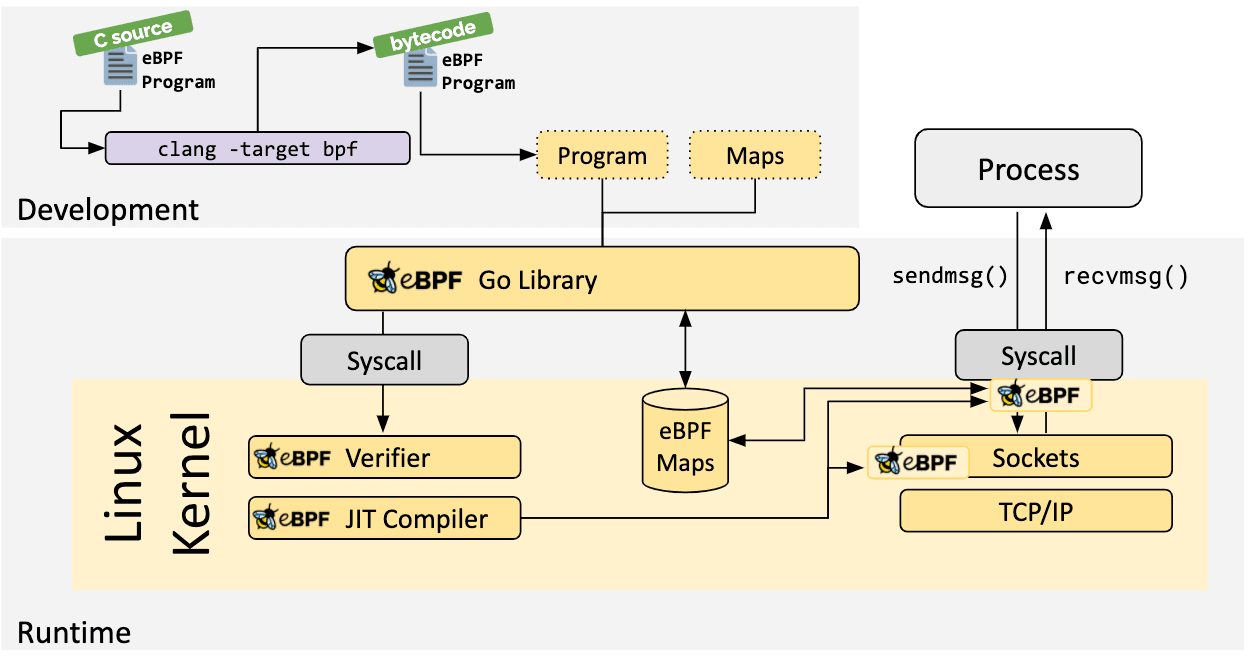
\includegraphics[width=0.9\textwidth]{ebpf.png}}
\caption{EBPF Architecture}
\label{fig:ebpf_architecture}
\end{figure}

Figure~\ref{fig:ebpf_architecture} illustrates the complete development-to-runtime workflow of an eBPF-based system. The numbered components below correspond to the stages shown in the figure.

\begin{enumerate}

\item \textbf{C Source eBPF Program.}
The eBPF program is initially written in C language. This source code defines the packet filtering logic, hook points, and data collection mechanisms. Since eBPF has strict safety constraints, only a limited subset of C is supported. A minimal example that counts \texttt{execve} system calls is shown in Listing~\ref{lst:ebpf-sample}.

\begin{lstlisting}[language=C,caption={Minimal eBPF C program: counting execve calls},label={lst:ebpf-sample}]
#include <linux/bpf.h>
#include <bpf/bpf_helpers.h>

struct {
    __uint(type, BPF_MAP_TYPE_ARRAY);
    __uint(max_entries, 1);
    __type(key,   __u32);
    __type(value, __u64);
} exec_count SEC(".maps");

SEC("tracepoint/syscalls/sys_enter_execve")
int count_exec(void *ctx)
{
    __u32 key = 0;
    __u64 *val = bpf_map_lookup_elem(&exec_count, &key);
    if (val)
        __sync_fetch_and_add(val, 1);
    return 0;
}

char LICENSE[] SEC("license") = "GPL";
\end{lstlisting}

\item \textbf{Clang/LLVM Compiler (\texttt{clang -target bpf}).}
The C source code is compiled using the LLVM-based \texttt{clang} compiler with the \texttt{-target bpf} option. This converts the high-level C program into eBPF bytecode, which is a hardware-independent instruction format targeting the eBPF virtual processor.

\item \textbf{eBPF Bytecode Program.}
The compiled eBPF bytecode is the verified instruction set loaded into the kernel. The eBPF virtual processor is a register-based machine with eleven 64-bit registers, a 512-byte stack, and a fixed instruction encoding. Unlike native code, bytecode is architecture-neutral and can be verified for safety before execution. The snippet below shows the bytecode disassembly corresponding to the map-lookup call in the sample program above:

\begin{lstlisting}[language={}]
; __u64 *val = bpf_map_lookup_elem(&exec_count, &key);
 0: r1 = exec_count         ; map file descriptor (rewritten at load)
 1: r2 = r10                ; frame pointer
 2: r2 += -4                ; &key on stack
 3: call bpf_map_lookup_elem
\end{lstlisting}

\item \textbf{Program and Maps.}
The \textbf{Program} refers to the loaded eBPF bytecode logic, while \textbf{Maps} are kernel-resident key--value data structures used for communication between kernel space and user space. Maps store packet metadata, statistics, and runtime state information. Example key--value pairs stored in the \texttt{exec\_count} array map: \texttt{key=0 \textrightarrow{} value=42} (total execve calls); in a per-UID hash map used by Execguard: \texttt{key=10123 \textrightarrow{} \{count=7, window\_start\_ns=168...\}}.

\item \textbf{eBPF Go Library.}
The eBPF Go library serves as the user-space control interface. It loads eBPF programs into the kernel, manages eBPF maps, and handles interaction between the user application and kernel space using system calls. (In this project the equivalent C library, \texttt{libbpf}, is used instead of the Go library.)

\item \textbf{System Call Interface.}
System calls act as the primary communication bridge between user space and kernel space. They are used to load eBPF programs, attach them to hooks, and perform read/write operations on eBPF maps.

\item \textbf{Linux Kernel eBPF Verifier.}
Once the program enters the kernel, it is first inspected by the eBPF verifier. The verifier performs strict safety checks to ensure the program cannot cause infinite loops, invalid memory access, or unsafe kernel behavior. Only verified programs are allowed to execute.

\item \textbf{eBPF JIT Compiler.}
After verification, the Just-In-Time (JIT) compiler translates the eBPF bytecode into native machine instructions for the processor of the target device. On the Motorola G96 5G used in this project the target is an AArch64 (ARM 64-bit) processor, so the JIT emits AArch64 machine code. This native compilation step eliminates the interpretation overhead that would otherwise apply to each bytecode instruction, making eBPF programs execute at near-native speed.

\item \textbf{eBPF Maps (Kernel Space).}
Kernel-resident eBPF maps serve as shared memory between kernel and user space. They store captured TCP packet metadata and are accessed both by the eBPF program and the Go user-space application.

\item \textbf{Process and Message Transfer.}
The user-space process communicates with the kernel through \texttt{sendmsg()} and \texttt{recvmsg()} system calls. These calls trigger the socket-level eBPF hooks, allowing real-time packet inspection and metadata extraction.

\end{enumerate}

Overall, the figure demonstrates the full lifecycle of an eBPF-based TCP monitoring system, from C source compilation and kernel verification to runtime packet capture at the IP layer and data retrieval in user space.

\noindent
In this project, eBPF is adopted as the primary kernel-level observability mechanism to analyze inter- and intra-process communication, packet flow behavior, and system-level vulnerabilities. By leveraging eBPF, the study aims to bridge the observability gap between conventional Linux systems and the constrained Android kernel environment.


\section{eBPF Evolution and CO-RE}
eBPF evolved from the classic Berkeley Packet Filter (cBPF) originally designed for network packet filtering into a general-purpose in-kernel virtual machine capable of safely executing user-defined programs at kernel event sites. The eBPF virtual machine is a sandboxed execution environment embedded in the kernel: it defines a register-based instruction set (eleven 64-bit registers, a 512-byte stack, and a compact fixed-width instruction encoding), a verifier that statically checks all programs for safety before they run, and a JIT compiler that translates the verified bytecode into native machine code for the host CPU. Programs run in this sandboxed context cannot crash the kernel, access arbitrary memory, or spin in infinite loops---properties the verifier enforces at load time. The verifier ensures program safety at load time, and an in-kernel JIT compiler converts approved programs to native machine code for near-zero overhead execution. Modern kernels provide BTF (BPF Type Format) metadata and the CO-RE (Compile Once, Run Everywhere) framework to adapt BPF programs to kernel data structure changes across versions without recompilation.\cite{mccanne1993bpf,starovoitov_bpf,ebpf_linux_doc,libbpf_doc} This is especially important for Android, where the adoption of the Generic Kernel Image (GKI) from Android 12 onward means kernel binaries are standardised across devices, making CO-RE-based programs more portable than kernel-module solutions.

\section{Linux Tracing Tools}
Traditional tracing tools offer powerful capabilities but come with significant limitations on Android. \texttt{strace} intercepts every syscall via \texttt{ptrace}, introducing overhead proportional to syscall frequency and making it impractical for continuous production monitoring. \texttt{ftrace} provides kernel-level function tracing but requires \texttt{debugfs} to be mounted, which is not guaranteed in restricted Android environments. \texttt{perf} is a capable sampling profiler but assumes a standard Linux distribution with perf support compiled in and a writable filesystem for recording. \texttt{bpftrace} and the BCC toolkit require LLVM to be present at runtime for JIT compilation of BPF programs from scripts, and neither LLVM nor BCC's Python dependencies are available in a standard Android environment.\cite{strace_doc,ftrace_doc,perf_doc,bpftrace_doc} These constraints motivate a pre-compiled, statically linked eBPF approach that can run inside a bootstrapped userspace\footnote{A \emph{bootstrapped userspace} is a minimal Linux root filesystem constructed from scratch on the target device using a tool such as \texttt{debootstrap}. It provides standard Linux utilities, libraries, and a package manager inside a directory tree that can be entered via \texttt{chroot}, without replacing or modifying the host Android system image.} without system-level package dependencies.

\section{Android Observability Tools}
Android provides Perfetto for system tracing and simpleperf for CPU profiling, both integrated into AOSP and designed for developer use \cite{android_perfetto, android_simpleperf, androidkernel2020}. Perfetto excels at scheduling, memory, and power traces but is oriented around performance analysis rather than security monitoring. simpleperf provides sampling-based CPU profiling but does not expose kernel event semantics such as process credential changes or VFS-level file operations. Neither tool is designed for continuous, low-noise security telemetry or for detecting behavioural anomalies at the process and privilege level.

\section{Security Monitoring Frameworks}
Modern security frameworks such as Falco~\cite{falco_doc}, Tetragon~\cite{tetragon_doc}, and Tracee~\cite{tracee_doc} leverage kernel signals and eBPF to detect suspicious behaviour on Linux systems. Falco attaches to kernel system call events and evaluates them against a rule engine. Tetragon, developed by the Cilium project~\cite{tetragon_doc}, offers fine-grained process and network policy enforcement via eBPF. Tracee by Aqua Security~\cite{tracee_doc} provides runtime forensics with a rich event model. However, all three assume a server-class Linux environment: they depend on \texttt{systemd}, package managers, container runtimes, or kernel features (such as LSM hooks---Linux Security Module~\cite{smalley2013security} hooks that allow eBPF programs to enforce security policy---or full BTF---BPF Type Format, the kernel metadata used for CO-RE relocations---exposure) that are not present on Android. Deploying these frameworks on Android would require porting significant infrastructure. Recent academic work validates the eBPF approach more broadly: Nelson et al.~formalise the correctness of BPF JIT compilers~\cite{bpf_jit_osdi2020}, and Li et al.~demonstrate eBPF-accelerated distributed protocols~\cite{electrode_nsdi2023}, collectively establishing eBPF as a reliable and performant platform for kernel-level tooling.

\section{Summary and Gap}
Existing tools demonstrate that kernel-level telemetry is valuable for security and debugging, but a clear gap remains: there are no lightweight, Android-oriented, verifier-friendly utilities that deliver focused security signals with minimal dependencies. The present work addresses this gap by providing a pre-compiled suite tuned to Android kernel constraints, deployable inside a bootstrapped Debian filesystem on the device without requiring LLVM or system-level packages.

\begin{table}[H]
  \centering
  \caption{Comparison of our approach with existing tools}
  \begin{tabular}{|p{0.20\textwidth}|p{0.18\textwidth}|p{0.18\textwidth}|p{0.18\textwidth}|p{0.16\textwidth}|}
    \hline
    \textbf{Tool/Approach} & \textbf{Overhead} & \textbf{Android Friendly} & \textbf{Kernel Signals} & \textbf{Focus} \\ \hline
    strace & High & Low & Syscalls & Debugging \\ \hline
    ftrace/perf & Medium & Medium & Kernel events & Performance \\ \hline
    bpftrace/BCC & Medium & Low & eBPF events & General tracing \\ \hline
    Falco & Medium-High & Low & Security events & Detection \\ \hline
    Aether & Low & High & Targeted events & Sec./Obs. \\ \hline
  \end{tabular}
\end{table}

\clearpage
\chapter{Background and Theoretical Foundation}
This section provides the technical background required to understand the design and implementation choices made across the suite. It covers the eBPF architecture and verifier model, the program types and hook points used in this project, the CO-RE portability framework, the ring buffer event delivery mechanism, Android's kernel constraints under the Generic Kernel Image model, and the Debian filesystem bootstrap that enables the development toolchain to run on the device.

\section{eBPF Architecture}
eBPF programs run in a restricted virtual machine embedded inside the Linux kernel. Before any program is executed, the kernel's verifier performs a static analysis pass to enforce safety properties: all memory accesses must be explicitly bounds-checked, loops must have a provably bounded iteration count, and the total stack frame is limited to 512 bytes. Programs that pass verification are JIT-compiled to native machine code and loaded into the kernel. BPF maps provide persistent, kernel-managed data structures (hash maps, arrays, ring buffers) that allow the kernel-side program and user-space process to exchange data efficiently.\cite{ebpf_linux_doc} The 512-byte stack limit is a practical constraint that shapes the design of every event struct in this suite: fields must be carefully sized and bounded arrays kept small to stay within budget.

\section{Program Types and Hook Points}
eBPF supports multiple program types, each suited to a different class of kernel event. This project uses three, whose characteristics and selection criteria are summarised below:

\begin{itemize}
  \item \textbf{Tracepoints} are statically defined, stable instrumentation points in the kernel source. They provide structured context (typed argument structs) and are preferred wherever available because they are part of the stable kernel ABI (Application Binary Interface---the set of kernel interfaces that are guaranteed not to change across minor kernel versions). \emph{Best suited for:} process lifecycle events (\texttt{sched\_process\_exec/fork/exit}), syscall entry/exit, and other well-specified kernel events. Used by Procwatch and Execguard in this project.

  \item \textbf{kprobes} are dynamic probes that attach to arbitrary kernel function entry or return points. They offer access to the exact function arguments and return values but are \emph{not} part of the stable ABI and may silently stop firing if the target function is inlined by the compiler or renamed across kernel versions. \emph{Best suited for:} internal kernel functions that have no corresponding tracepoint, such as \texttt{commit\_creds} (privilege changes) and VFS functions (\texttt{vfs\_open}, \texttt{vfs\_write}). Used by Priviwatch and Filewatch in this project.

  \item \textbf{TC ingress} is a traffic-control hook that fires on inbound (and, in the extended version, outbound) packets after \texttt{sk\_buff} allocation but before the network stack's upper layers process them. It provides access to the raw socket buffer and is compatible with virtualised and Wi-Fi network interfaces. Unlike XDP---eXpress Data Path, a lower-level driver hook described in Chapter~\ref{ch:design}---TC ingress does not require explicit driver support. \emph{Best suited for:} packet inspection and lightweight filtering without needing to drop or modify packets. Used by Pktrace in this project.
\end{itemize}

Table~\ref{tab:hookpoint-comparison} summarises the key differences across the three hook types.

\begin{table}[H]
  \centering
  \caption{Comparison of eBPF hook point types used in this project}
  \label{tab:hookpoint-comparison}
  \begin{tabular}{|p{0.18\textwidth}|p{0.18\textwidth}|p{0.18\textwidth}|p{0.18\textwidth}|p{0.16\textwidth}|}
    \hline
    \textbf{Property} & \textbf{Tracepoint} & \textbf{kprobe} & \textbf{TC ingress} \\ \hline
    Stability & Stable ABI & Not stable ABI & Stable (tc subsystem) \\ \hline
    Argument access & Typed struct & Raw registers & sk\_buff pointer \\ \hline
    Inlining risk & None & Yes & N/A \\ \hline
    Typical use & Process events & Internal functions & Packet inspection \\ \hline
    Tools in this project & Procwatch, Execguard & Priviwatch, Filewatch & Pktrace \\ \hline
  \end{tabular}
\end{table}

\section{CO-RE and BTF}
CO-RE (Compile Once, Run Everywhere) allows a BPF object compiled on a development machine to adapt to the kernel data structure layout of the target device at load time, without requiring recompilation. The mechanism relies on BTF (BPF Type Format)---a compact type-description format embedded in the kernel image that encodes the names, types, and byte offsets of every kernel data structure. When an eBPF program uses \texttt{BPF\_CORE\_READ} to read a field from a kernel struct, the compiler annotates the instruction with a relocation record. At load time, \texttt{libbpf} reads the BTF from the running kernel, looks up the actual byte offset of the requested field in \emph{that} kernel's layout, and patches the instruction accordingly. The net effect is that a single compiled binary works correctly even when the field moves to a different offset in a newer or older kernel build~\cite{libbpf_doc}.

On Android, BTF availability varies: GKI kernels from Android 13 onward generally include it, but older images or custom builds may not expose BTF for all struct types. \emph{Unreliability} in this context means that \texttt{libbpf} encounters a CO-RE relocation targeting a type or field absent from the device's BTF, causing the load to abort with a relocation error. Where such unreliability occurs---as was the case for Priviwatch~(Section~\ref{sec:priviwatch})'s access to the capability fields inside \texttt{struct cred}---the fallback is \texttt{bpf\_probe\_read\_kernel} into a locally defined struct that mirrors the expected memory layout, bypassing CO-RE entirely. This trades some portability for reliable load-time behaviour on the specific kernel.

\section{Ring Buffer vs Perf Buffer}
The suite uses BPF ring buffers (\texttt{BPF\_MAP\_TYPE\_RINGBUF}) exclusively for event delivery rather than the older perf event arrays (\texttt{BPF\_MAP\_TYPE\_PERF\_EVENT\_ARRAY}). Perf event arrays require per-CPU buffer allocation, which wastes memory on multi-core devices and complicates the user-space polling loop. Ring buffers use a single shared memory region with a simpler API: \texttt{bpf\_ringbuf\_reserve} reserves a slot, the program fills it, and \texttt{bpf\_ringbuf\_submit} makes it visible. On the user-space side, \texttt{ring\_buffer\_\_poll} is a single blocking call that \emph{drains} (reads and processes) all pending events---that is, it invokes the registered callback for every event slot that the kernel side has submitted and not yet consumed, then marks those slots as free. Events are delivered in submission order; no events are discarded by the drain operation itself. Events may, however, be lost earlier---at production time---if the kernel-side program attempts to reserve a slot when the ring buffer is already full; in that case the reservation fails and the event is silently dropped, incrementing an internal drop counter. This design also provides natural backpressure: if the ring buffer fills, events are dropped and a drop counter is incremented, making it straightforward to measure the drop rate.

\section{Android Kernel Specifics}
Android's Generic Kernel Image (GKI), introduced in Android 12, standardises the kernel binary across hardware platforms so that OEMs can no longer patch the upstream kernel arbitrarily. One consequence is that loadable kernel modules are restricted or prohibited unless signed by Google: a vendor cannot ship a kernel module that was not part of the original GKI build. This makes eBPF one of the very few mechanisms available for extending kernel behaviour or observing kernel internals on a production Android device without modifying the system image. GKI kernels are also required to enable a set of eBPF-relevant config options (\texttt{CONFIG\_BPF}, \texttt{CONFIG\_BPF\_SYSCALL}, \texttt{CONFIG\_BPF\_JIT}), making the eBPF subsystem reliably present from Android 12 onward.\cite{android_gki,android_ebpf_monitor}

\section{Debian Filesystem Bootstrap}
The Android device does not include a full Linux development environment by default. The Android shell provides only \texttt{toybox} utilities and does not ship clang, libbpf, bpftool, or standard build infrastructure. To provide these tools, a Debian GNU/Linux~11 (bullseye) root filesystem was constructed inside the rooted device\footnote{All development and testing was performed on a physical Motorola G96~5G device running a rooted Android image. Initial exploration used an Android emulator, but all final tool validation and the performance measurements reported in Chapter~\ref{ch:results} were conducted on the physical device.} using \texttt{debootstrap}\footnote{\texttt{debootstrap} is the standard Debian/Ubuntu tool for constructing a minimal Debian root filesystem from the package repository without needing an existing Debian installation.} and made accessible through a \texttt{chroot} environment. This is a well-established technique among Android security researchers for deploying standard Linux toolchains on physical devices without replacing or modifying the Android system image or partition layout.

The step-by-step procedure to reproduce this environment is as follows:

\begin{enumerate}
  \item \textbf{Obtain a rooted device and enable ADB.} Unlock the bootloader of the Motorola G96~5G, flash a root-enabled system image, and enable USB debugging in Developer Options.

  \item \textbf{Push \texttt{debootstrap} to the device.}
  \begin{lstlisting}[language=bash]
adb push debootstrap /data/local/tmp/
adb shell chmod +x /data/local/tmp/debootstrap
  \end{lstlisting}

  \item \textbf{Create a target directory and run \texttt{debootstrap}.}
  \begin{lstlisting}[language=bash]
adb shell mkdir -p /data/debian
adb shell /data/local/tmp/debootstrap \
    --arch=arm64 --foreign bullseye \
    /data/debian http://deb.debian.org/debian
  \end{lstlisting}

  \item \textbf{Complete the second-stage bootstrap inside the device.}
  \begin{lstlisting}[language=bash]
adb shell chroot /data/debian /debootstrap/debootstrap \
    --second-stage
  \end{lstlisting}

  \item \textbf{Mount required pseudo-filesystems and enter the chroot.}
  \begin{lstlisting}[language=bash]
adb shell mount --bind /dev  /data/debian/dev
adb shell mount --bind /proc /data/debian/proc
adb shell mount --bind /sys  /data/debian/sys
adb shell mount -t debugfs debugfs \
    /sys/kernel/debug
adb shell mount --bind /sys/kernel/debug \
    /data/debian/sys/kernel/debug
adb shell chroot /data/debian /bin/bash
  \end{lstlisting}

  \item \textbf{Install the build toolchain inside the chroot.}
  \begin{lstlisting}[language=bash]
apt-get update
apt-get install -y clang llvm libbpf-dev linux-tools-common \
    linux-headers-$(uname -r) gcc make
  \end{lstlisting}
\end{enumerate}

Within this Debian environment, the full build toolchain is available: clang~11.0.1, bpftool~5.10.223, libbpf, and gcc. All eBPF programs in this suite are compiled and loaded from within this Debian chroot, while the Android kernel itself provides the execution environment for the loaded programs. Appendix~\ref{app:ebpf} lists the key configuration options and commands required.

Figure~\ref{fig:ebpf-pipeline} illustrates the five-stage pipeline through which every eBPF program passes before it can execute on kernel events. The eBPF source is compiled to bytecode by clang/LLVM, the kernel verifier performs a static safety analysis, the JIT compiler emits native machine code, the program is attached to its chosen hook point, and from that moment onward it fires automatically on each matching kernel event.

\begin{figure}[H]
  \centering
  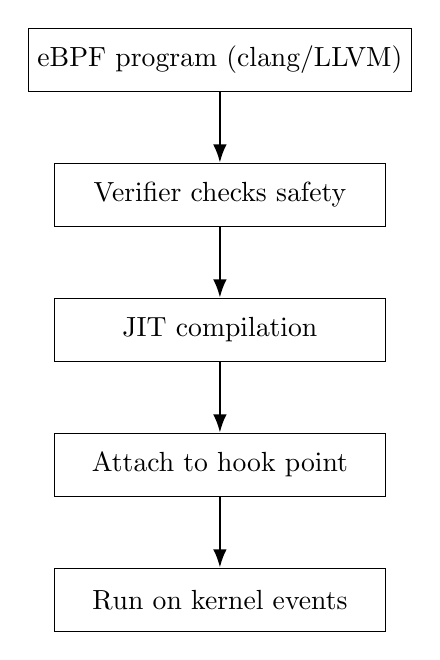
\begin{tikzpicture}[
    node distance=0.9cm,
    box/.style={rectangle, draw, align=center, minimum width=4.2cm, minimum height=0.8cm},
    arrow/.style={-Latex, thick}
  ]
    \node[box] (prog) {eBPF program (clang/LLVM)};
    \node[box, below=of prog] (verifier) {Verifier checks safety};
    \node[box, below=of verifier] (jit) {JIT compilation};
    \node[box, below=of jit] (attach) {Attach to hook point};
    \node[box, below=of attach] (run) {Run on kernel events};
    \draw[arrow] (prog) -- (verifier);
    \draw[arrow] (verifier) -- (jit);
    \draw[arrow] (jit) -- (attach);
    \draw[arrow] (attach) -- (run);
  \end{tikzpicture}
  \caption{Simplified eBPF verification and execution pipeline.}
  \label{fig:ebpf-pipeline}
\end{figure}

\clearpage
\chapter{Tools and Techniques}
This project uses open source tooling to compile, load, and attach eBPF programs. Each component plays a specific role in the build and deployment pipeline. This section describes the four core infrastructure tools used, the Makefile structure and skeleton generation pipeline they enable, and the user-space loader pattern common to all five monitoring utilities (Procwatch, Execguard, Priviwatch, Filewatch, and Pktrace) described in Chapter~\ref{ch:implementations}.

\begin{itemize}
  \item \textbf{clang/llvm}: compiles BPF C source to BPF bytecode targeting the \texttt{bpf} architecture. The BPF backend in LLVM generates bytecode that the kernel verifier can analyse.
  \item \textbf{libbpf}: the primary library for loading and managing BPF objects. It handles CO-RE relocations at load time, manages map creation and attachment, and provides the ring buffer polling API.
  \item \textbf{bpftool}: a multi-purpose BPF utility used here primarily to generate C skeleton headers (\texttt{bpftool gen skeleton}). Skeletons provide a typed, auto-generated interface for opening, loading, attaching, and destroying a BPF object from user-space C code.
  \item \textbf{adb}: the Android Debug Bridge, used to push binaries to the device and execute commands in the Android environment from the host terminal.
\end{itemize}

\section{Makefile Structure and Skeleton Generation}
Each tool's Makefile follows a shared three-stage pipeline. First, the BPF C source is compiled with clang targeting the \texttt{bpf} architecture to produce a \texttt{.o} object file. Second, \texttt{bpftool gen skeleton} reads that object and generates a \texttt{.skel.h} header containing a typed C struct that wraps the BPF maps and programs, along with helper functions to open, load, attach, and destroy the object. Third, the user-space C program is compiled against libbpf and the generated skeleton header to produce the final binary. This pipeline ensures that the user-space program has type-safe access to all BPF maps and programs without manual file descriptor management. All of this is summarised, along with the necessary commands, in Listing~\ref{lst:build-pipeline}.

\begin{lstlisting}[language=bash,caption={Typical build pipeline for each tool},label={lst:build-pipeline}]
# Stage 1: compile BPF program to bytecode
clang -O2 -g -target bpf -c tool.bpf.c -o tool.bpf.o

# Stage 2: generate skeleton header
bpftool gen skeleton tool.bpf.o > tool.skel.h

# Stage 3: compile user-space binary
gcc tool.c -o tool -lbpf
\end{lstlisting}

\section{User-space Loader and Poll Loop}
The user-space components follow a consistent pattern across all five tools. After skeleton open and load, the BPF programs are attached to their respective hook points. A ring buffer is created with a callback function registered to handle incoming events. The main loop calls \texttt{ring\_buffer\_\_poll} with a timeout, which blocks until events are available, then invokes the callback for each pending event. The callback formats and prints the event fields to stdout. This design keeps the user-space logic minimal and ensures that event processing stays close to the kernel delivery rate. Listing~\ref{lst:poll-loop} illustrates this process.

\begin{lstlisting}[language=C,caption={Generic user-space loader and poll loop pattern},label={lst:poll-loop}]
skel = tool_bpf__open_and_load();
tool_bpf__attach(skel);
rb = ring_buffer__new(bpf_map__fd(skel->maps.rb),
                      handle_event, NULL, NULL);
while (1) {
    ring_buffer__poll(rb, 100 /* ms timeout */);
}
\end{lstlisting}

Figure~\ref{fig:toolchain} shows the complete toolchain pipeline for all five monitoring utilities.

\begin{figure}[H]
  \centering
  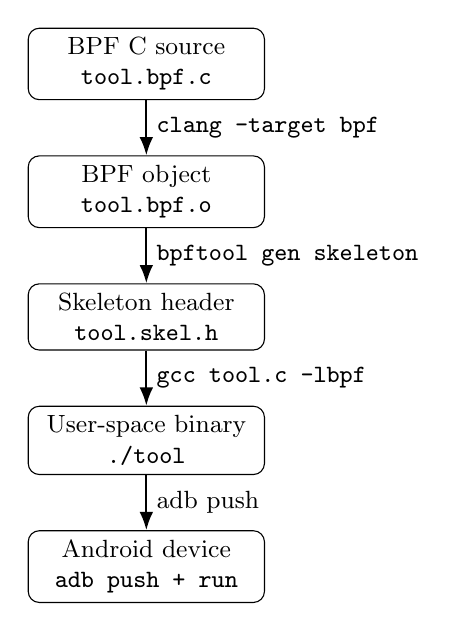
\begin{tikzpicture}[
    node distance=0.7cm and 1.2cm,
    box/.style={rectangle, draw, rounded corners, align=center,
                minimum width=3.0cm, minimum height=0.7cm, font=\small},
    arrow/.style={-Latex, thick}
  ]
    \node[box] (src)    {BPF C source\\\texttt{tool.bpf.c}};
    \node[box, below=of src] (obj)    {BPF object\\\texttt{tool.bpf.o}};
    \node[box, below=of obj] (skel)   {Skeleton header\\\texttt{tool.skel.h}};
    \node[box, below=of skel] (bin)   {User-space binary\\\texttt{./tool}};
    \node[box, below=of bin] (device) {Android device\\\texttt{adb push + run}};

    \draw[arrow] (src)  -- node[right,font=\small]{\texttt{clang -target bpf}} (obj);
    \draw[arrow] (obj)  -- node[right,font=\small]{\texttt{bpftool gen skeleton}} (skel);
    \draw[arrow] (skel) -- node[right,font=\small]{\texttt{gcc tool.c -lbpf}} (bin);
    \draw[arrow] (bin)  -- node[right,font=\small]{adb push} (device);
  \end{tikzpicture}
  \caption{Complete build and deployment toolchain for each of the five monitoring utilities.}
  \label{fig:toolchain}
\end{figure}

\clearpage
\chapter{Methodology}
\label{ch:methodology}
This section presents the overall data flow, system architecture, and event processing model used across the suite. It describes how kernel events generated by Android applications and system processes are intercepted by eBPF programs, structured into typed events, and delivered to user-space tools via ring buffers. The system architecture is presented first, followed by the common event flow shared by the five monitoring tools---Procwatch, Execguard, Priviwatch, Filewatch, and Pktrace---and a step-by-step summary of the processing pipeline.

\section{System Architecture}

Figure~\ref{fig:system-arch} shows the high-level architecture of the eBPF tool suite. Android user-space activity (apps, shell commands, system services) generates kernel events. The eBPF programs attached to tracepoints, kprobes, and TC hooks intercept these events inside the kernel. Each event is written to a per-tool BPF ring buffer map. The user-space component of each tool polls the ring buffer, formats the event fields, and produces structured output for the analyst.

\noindent
The architecture is intentionally layered: the kernel-space component is responsible only for minimal, safe data extraction; all interpretation, filtering, and alerting logic resides in user space. This division keeps the kernel footprint small and within verifier constraints.

\begin{figure}[H]
  \centering
  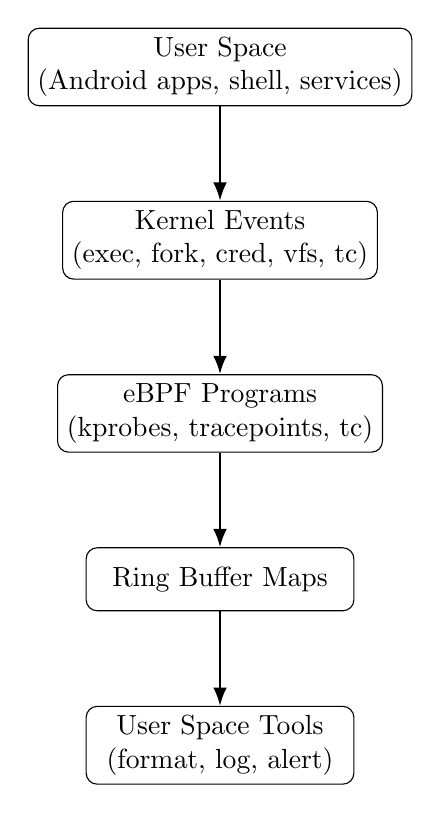
\begin{tikzpicture}[
    node distance=1.2cm,
    box/.style={rectangle, draw, rounded corners, align=center, minimum width=3.4cm, minimum height=0.8cm},
    arrow/.style={-Latex, thick}
  ]
    \node[box] (app) {User Space\\(Android apps, shell, services)};
    \node[box, below=of app] (kernel) {Kernel Events\\(exec, fork, cred, vfs, tc)};
    \node[box, below=of kernel] (bpf) {eBPF Programs\\(kprobes, tracepoints, tc)};
    \node[box, below=of bpf] (rb) {Ring Buffer Maps};
    \node[box, below=of rb] (user) {User Space Tools\\(format, log, alert)};
    \draw[arrow] (app) -- (kernel);
    \draw[arrow] (kernel) -- (bpf);
    \draw[arrow] (bpf) -- (rb);
    \draw[arrow] (rb) -- (user);
  \end{tikzpicture}
  \caption{System architecture of the eBPF tool suite.}
  \label{fig:system-arch}
\end{figure}

% \section{Common Event Flow}
% \begin{figure}[H]
%   \centering
%   \begin{tikzpicture}[
%     node distance=0.9cm,
%     box/.style={rectangle, draw, align=center, minimum width=4.2cm, minimum height=0.8cm},
%     arrow/.style={-Latex, thick}
%   ]
%     \node[box] (event) {Kernel event occurs};
%     \node[box, below=of event] (probe) {Probe validates and reads metadata};
%     \node[box, below=of probe] (filter) {Filter/threshold (optional)};
%     \node[box, below=of filter] (emit) {Emit event to ring buffer};
%     \node[box, below=of emit] (poll) {User space polls and formats output};
%     \draw[arrow] (event) -- (probe);
%     \draw[arrow] (probe) -- (filter);
%     \draw[arrow] (filter) -- (emit);
%     \draw[arrow] (emit) -- (poll);
%   \end{tikzpicture}
%   \caption{Generic event processing flow used across the tools.}
%   \label{fig:event-flow}
% \end{figure}

\section{Algorithmic Summary}
The following steps describe the common processing pipeline shared by all five tools (Procwatch, Execguard, Priviwatch, Filewatch, and Pktrace). Each tool implements this pipeline independently; the hook point and event struct differ per tool, but the overall flow is identical.

Table~\ref{tab:hook-coverage} enumerates the eBPF filter attachment points available in the Linux/Android kernel and indicates which of the five tools covers each point, demonstrating the breadth of observability achieved.

\begin{table}[H]
  \centering
  \caption{eBPF filter attachment points and tool coverage}
  \label{tab:hook-coverage}
  \begin{tabular}{|p{0.28\textwidth}|p{0.28\textwidth}|p{0.32\textwidth}|}
    \hline
    \textbf{Attachment Point} & \textbf{Event Type} & \textbf{Covered by} \\ \hline
    \texttt{sched\_process\_exec} tracepoint & Process exec & Procwatch, Execguard \\ \hline
    \texttt{sched\_process\_fork} tracepoint & Process fork & Procwatch \\ \hline
    \texttt{sched\_process\_exit} tracepoint & Process exit & Procwatch \\ \hline
    \texttt{commit\_creds} kprobe & Credential change & Priviwatch \\ \hline
    \texttt{vfs\_open} kprobe & File open & Filewatch \\ \hline
    \texttt{vfs\_write} kprobe & File write & Filewatch \\ \hline
    \texttt{vfs\_unlink} kprobe & File delete & Filewatch \\ \hline
    \texttt{vfs\_rename} kprobe & File rename & Filewatch \\ \hline
    TC ingress / TC egress & Inbound/outbound packets & Pktrace \\ \hline
    Syscall entry/exit tracepoints & Individual system calls & Not covered (future work) \\ \hline
    LSM (Linux Security Module) hooks & Policy enforcement events & Not covered (future work) \\ \hline
  \end{tabular}
\end{table}
\begin{enumerate}
  \item Attach probes to the chosen hook point (tracepoints, kprobes, or TC ingress).
  \item Validate all memory accesses and enforce bounds at the BPF program level to satisfy the verifier.
  \item Extract key fields (pid, uid, comm, inode, ports, etc.) from kernel data structures via \texttt{BPF\_CORE\_READ} or \texttt{bpf\_probe\_read\_kernel}.
  \item Apply minimal filters (e.g., emit only on credential changes, only regular files, only IPv4).
  \item Reserve a slot in the ring buffer, populate the event struct, and submit.
  \item User space polls the ring buffer, formats the event fields, and prints or logs output.
\end{enumerate}

\clearpage
\chapter{Design Decisions and Architecture}
\label{ch:design}
This section explains the key architectural choices made during the design of the suite. Each decision involves a tradeoff that was evaluated in the context of Android's constraints and the observability goals of the project. The five tools appear in the following sequence in the monitoring toolchain: (1)~Procwatch monitors process lifecycle; (2)~Execguard aggregates exec-rate anomalies; (3)~Priviwatch detects privilege transitions; (4)~Filewatch tracks VFS-level file operations; and (5)~Pktrace captures network packets. The subsections below cover the rationale for this modular approach, the choice of ring buffers over perf event arrays, the selection of TC ingress over XDP for packet capture, and the fixed-size event struct design that satisfies verifier constraints.

\section{Why Separate Tools}
The suite is implemented as five focused, independent utilities rather than a single monolithic agent. A monolithic design would combine all hook points into one BPF object, increasing the verifier surface area and making failures harder to isolate. If a single large program fails verification on a particular kernel configuration, the entire monitoring capability is lost. Independent tools can be loaded, tested, and validated one at a time, which proved essential during development on the Motorola G96 5G where verifier behaviour differed from desktop Linux. The modular design also allows each tool to be deployed selectively: an analyst investigating a privilege escalation may only need Priviwatch~(Section~\ref{sec:priviwatch}) and Procwatch~(Section~\ref{sec:procwatch}), without loading file or network monitoring overhead. Maintenance and iteration are also simplified since a change to Pktrace's packet parsing logic cannot affect Execguard's exec-rate tracking.

\section{Why Ring Buffers}
The suite standardises on BPF ring buffers (\texttt{BPF\_MAP\_TYPE\_RINGBUF}) rather than the older perf event arrays (\texttt{BPF\_MAP\_TYPE\_PERF\_EVENT\_ARRAY}). Perf event arrays require a separate buffer per logical CPU core, which means the user-space polling loop must open and poll a file descriptor for each CPU — a significant setup overhead on a multi-core device. Ring buffers use a single shared memory region regardless of CPU count, and the user-space API reduces to a single \texttt{ring\_buffer\_\_poll} call. For the event rates observed in this project (tens to a few hundred events per second), the ring buffer's capacity is more than sufficient and its simpler semantics reduce the risk of implementation bugs in the polling loop.

The key ring buffer API methods and their semantics are listed in Table~\ref{tab:ringbuf-api}.

\begin{table}[H]
  \centering
  \small
  \caption{BPF ring buffer API methods}
  \label{tab:ringbuf-api}
  \begin{tabular}{|p{0.30\textwidth}|p{0.60\textwidth}|}
    \hline
    \textbf{Method} & \textbf{Description} \\ \hline
    \texttt{bpf\_ringbuf\_reserve(\allowbreak rb,\allowbreak size,\allowbreak flags)} & Atomically reserves \texttt{size} bytes in the ring buffer \texttt{rb}. Returns a pointer to the reserved slot, or \texttt{NULL} if the buffer is full. The event struct is filled in place via the returned pointer. \\ \hline
    \texttt{bpf\_ringbuf\_submit(\allowbreak data,\allowbreak flags)} & Marks the previously reserved slot as ready for user-space consumption. After this call the slot is visible to \texttt{ring\_buffer\_\_poll}. \\ \hline
    \texttt{bpf\_ringbuf\_discard(\allowbreak data,\allowbreak flags)} & Cancels a reservation without emitting an event. Used when a filter condition is not met after the slot was reserved. \\ \hline
    \texttt{ring\_buffer\_\_new(\allowbreak fd,\allowbreak cb,\allowbreak ctx,\allowbreak opts)} & User-space: creates a ring buffer consumer backed by the BPF map file descriptor \texttt{fd}, registering \texttt{cb} as the per-event callback. \\ \hline
    \texttt{ring\_buffer\_\_poll(\allowbreak rb,\allowbreak timeout\_ms)} & User-space: blocks for up to \texttt{timeout\_ms} milliseconds, then invokes the callback for every pending event in submission order, draining the buffer. Returns the number of events processed. \\ \hline
  \end{tabular}
\end{table}

\section{Why TC Ingress (Not XDP)}
XDP (eXpress Data Path) is an eBPF hook point that operates at the lowest level of the network stack---at the network driver layer, before the kernel allocates an \texttt{sk\_buff} structure for the packet. Because it fires so early, XDP can forward, drop, or redirect packets with the lowest possible latency. However, XDP is not part of eBPF per se; it is an optional driver-level feature. A network interface can only support XDP if its driver has been explicitly written to expose the XDP hook, which is not guaranteed on all hardware. XDP is an alternative to TC ingress, not a component of it; both are eBPF attachment points but at different layers of the Linux network stack.

On the Motorola G96 5G used in this project, the active network interface does not expose an XDP hook in the Android kernel configuration, making XDP unavailable. TC ingress operates one layer up, on the \texttt{sk\_buff} after it has been allocated, which makes packet metadata (length, protocol, headers) accessible via the standard \texttt{bpf\_skb\_load\_bytes} API. TC ingress is also available on all interface types including Wi-Fi and mobile data (rmnet) adapters that are common on Android devices. TC ingress is also sufficient for the inspection use case: Pktrace does not need to modify or drop packets, so the minimal additional latency of TC versus XDP is irrelevant.

\section{Event Struct Design}
All event structs are fixed-size with bounded arrays. This is not purely a style choice: the BPF verifier requires that all memory writes to a reserved ring buffer slot be bounded at compile time. Variable-length data (such as full command-line arguments or complete file paths) would require dynamic allocation patterns that either exceed the 512-byte stack limit or require loop constructs the verifier may reject. Fixed-size structs also make \texttt{bpf\_ringbuf\_reserve} straightforward — the size argument is always \texttt{sizeof(struct event)}, which is a compile-time constant. The tradeoff is that long strings are truncated at the array boundary, but for the fields captured here (process name, filename component, payload preview) the bounded sizes are sufficient for the intended use cases.

\clearpage
\chapter{Tool Implementations}
\label{ch:implementations}
This section describes each of the five tools in detail. For each tool, the discussion covers the design motivation, the kernel hook point chosen and the reasoning behind it, the event structure sent to user space, the key filtering and logic implemented in the BPF program, security use cases illustrating how the tool applies to real attack scenarios, output interpretation guidance, usage notes, and known limitations. Screenshots of test commands and tool output are included at the end of each subsection.

\section{Procwatch}
\label{sec:procwatch}
\textbf{Motivation:} Observe process lifecycle at the kernel level to detect short-lived processes, rapid forks, and suspicious exec patterns. Procwatch provides the foundational process context that gives meaning to later signals from Priviwatch, Filewatch, and Pktrace. Without knowing which process performed a privilege change or opened a sensitive file, the other tools produce signals without attribution.

\textbf{Hook points:} Three tracepoints provide stable, structured event context across kernels:\linebreak
\texttt{sched\_process\_exec} fires when a process calls \texttt{execve} and the new binary is mapped; \texttt{sched\_process\_fork} fires when a new process is created; and \texttt{sched\_process\_exit} fires when a process exits. Tracepoints are preferred over kprobes here because the scheduling tracepoints are part of the stable kernel instrumentation interface and provide well-typed argument structs.

\textbf{Event structure:}
\begin{lstlisting}[language=C,caption={Procwatch event structure}]
struct event {
    u32 pid;
    u32 ppid;
    u32 uid;
    u32 gid;
    u32 inum;        /* namespace inode, identifies process namespace */
    int exit_code;
    u64 timestamp;
    u8  type;        /* EVENT_EXEC, EVENT_FORK, or EVENT_EXIT */
    char comm[TASK_COMM_LEN];
    char filename[MAX_FILENAME_LEN];
    char args[MAX_ARGS_LEN];
};
\end{lstlisting}

\textbf{Filtering and logic:} Procwatch emits one event per lifecycle transition. For exec events, the filename is read from the tracepoint context and a bounded argv buffer is read from user memory using \texttt{bpf\_probe\_read\_user}. Fork events capture the parent comm from the tracepoint context. Exit events extract the exit code from the task struct using CO-RE.

\textbf{Key logic snippets:}
\begin{lstlisting}[language=C,caption={Procwatch exec handler}]
SEC("tracepoint/sched/sched_process_exec")
int handle_exec(struct trace_event_raw_sched_process_exec *ctx)
{
    struct event *e = bpf_ringbuf_reserve(&rb, sizeof(*e), 0);
    if (!e) return 0;
    e->type = EVENT_EXEC;
    e->pid = bpf_get_current_pid_tgid() >> 32;
    bpf_get_current_comm(e->comm, sizeof(e->comm));
    /* read filename from tracepoint context */
    bpf_ringbuf_submit(e, 0);
    return 0;
}
\end{lstlisting}
\\.
\begin{lstlisting}[language=C,caption={Procwatch exit code extraction via CO-RE}]
e->exit_code = (BPF_CORE_READ(task, exit_code) >> 8) & 0xff;
\end{lstlisting}

\textbf{Security use cases:} Procwatch is the first tool to run in any investigation. By observing fork and exec sequences, an analyst can trace which binaries led to sensitive file or network activity. A compromised application spawning a reverse shell will appear as an EXEC event with \texttt{parent\_comm} matching the app process and \texttt{comm} showing \texttt{sh} or a similar interpreter. Rapid fork storms from a single parent PID are an early indicator of fork-bomb-style resource exhaustion or parallel exploit spawning. Combined with the namespace inode, Procwatch can distinguish activity across isolated process namespaces.

\textbf{Output interpretation:} A normal system shows steady EXEC and EXIT pairs for expected system binaries with exit code 0. Suspicious patterns include rapid fork storms from a single parent, frequent short-lived shells appearing with non-root UIDs, or repeated EXEC events from parents that have no business spawning child processes (e.g., a media decoder spawning a shell).

\textbf{Usage notes:} Procwatch is typically run first to build a baseline process timeline. In investigations, its parent-child output provides context for explaining later alerts from Priviwatch, Filewatch, or Pktrace. Running it alongside Execguard is particularly effective: Execguard counts exec bursts per UID, and Procwatch provides the exact filenames and parent chains responsible.

\textbf{Limitations:} Args capture is bounded by \texttt{MAX\_ARGS\_LEN} and may be truncated for long command lines. Fork events do not include the namespace inode in all kernel configurations due to tracepoint context availability.

\begin{figure}[H]
  \centering
  \includegraphics[width=1.05\linewidth]{\detokenize{Procwatch_Snapshot of commands ran.png}}
  \caption{Procwatch commands used during testing.}
  \label{fig:procwatch-commands}
\end{figure}

\begin{figure}[H]
  \centering
  \includegraphics[width=1.05\linewidth]{\detokenize{Procwatch_tool's output of the commands.png}}
  \caption{Procwatch output showing EXEC/FORK/EXIT events.}
  \label{fig:procwatch-output}
\end{figure}

\section{Execguard}
\textbf{Motivation:} Detect unusual execution behavior such as rapid command spawning or shell usage by non-root UIDs. While Procwatch observes every exec event individually, Execguard aggregates them over time to surface rate-based anomalies that would be invisible in a per-event stream. A script-based exploit chain typically involves executing tens or hundreds of binaries in quick succession; Execguard makes this pattern visible.

\textbf{Hook point:} Tracepoint \texttt{sched\_process\_exec} provides stable exec metadata across kernels. The same tracepoint used by Procwatch is reused here, with a different program logic focused on rate tracking rather than individual event capture.

\textbf{Event structure:}
\begin{lstlisting}[language=C,caption={Execguard event structure}]
struct event {
    __u32 pid;
    __u32 ppid;
    __u32 uid;
    __u32 exec_count;   /* cumulative exec count in current window */
    char  comm[TASK_COMM_LEN];
    char  parent_comm[TASK_COMM_LEN];
    char  binary_path[PATH_LEN];
};
\end{lstlisting}

\textbf{Filtering and logic:} Execguard maintains a per-UID sliding window using a BPF hash map keyed by UID. Each exec event increments the counter for the executing UID. If the elapsed time since the window start exceeds 60 seconds (\texttt{WINDOW\_NS}), the counter resets and a new window begins. The current exec count is embedded in each emitted event so the user-space component can apply severity labels without additional state.

\textbf{Key logic snippets:}
\begin{lstlisting}[language=C,caption={Execguard sliding window rate tracking}]
st = bpf_map_lookup_elem(&stats, &key);
if (!st) {
    init.window_start_ns = now;
    init.count = 1;
    bpf_map_update_elem(&stats, &key, &init, BPF_ANY);
    e->exec_count = 1;
} else {
    if (now - st->window_start_ns > WINDOW_NS) {
        st->window_start_ns = now;
        st->count = 1;
    } else {
        st->count++;
    }
    e->exec_count = st->count;
}
\end{lstlisting}

\begin{lstlisting}[language=C,caption={Execguard shell heuristic and severity labelling (user space)}]
if (is_shellish(base) && e->uid != 0)
    return "ALERT";
if (e->exec_count > HIGH_EXEC_THRESHOLD)
    return "WARN";
return "INFO";
\end{lstlisting}

\textbf{Security use cases:} A burst of shell invocations is a strong indicator of a dropper or script-based exploit chain. When a non-root UID repeatedly spawns shells or utility programs (\texttt{sh}, \texttt{toybox}, \texttt{su}), Execguard highlights the sequence with escalating severity labels. An attacker using a post-exploitation framework that stages payloads via shell scripts will produce a clear ALERT signal within the first few seconds of execution. The exec count provides a quantitative measure that can be correlated with specific time windows.

\textbf{Output interpretation:} INFO events represent individual exec events that are within normal rate bounds. WARN indicates elevated exec activity that may still be benign (e.g., an update script running). ALERT signals either a non-root UID spawning a shell-like binary, or an exec rate that exceeds the configured threshold. The exec count field tracks cumulative execs within the current 60-second window for the offending UID.

\textbf{Usage notes:} Execguard pairs well with Procwatch to identify the exact parent process responsible for an exec burst. In demonstrations, a short loop of \texttt{for i in \$(seq 1 50); do sh -c "echo x"; done} will rapidly escalate the severity label and demonstrate the windowing behaviour.

\textbf{Limitations:} The full command line is not captured because reading variable-length user-space memory in a loop is rejected by the verifier on some kernel configurations. Binary identity is derived from \texttt{comm}, which is limited to 15 characters and can be truncated for long binary names.

\begin{figure}[H]
  \centering
  \includegraphics[width=0.9\linewidth]{\detokenize{execguard_Snapshot of Commands ran.png}}
  \caption{Execguard commands used to trigger exec activity.}
  \label{fig:execguard-commands}
\end{figure}

\begin{figure}[H]
  \centering
  \includegraphics[width=0.9\linewidth]{\detokenize{execguard_tool's output for the commands ran.png}}
  \caption{Execguard output showing WARN/INFO events and exec counts.}
  \label{fig:execguard-output}
\end{figure}

\section{Priviwatch}
\label{sec:priviwatch}
\textbf{Motivation:} Detect privilege transitions at the exact moment credentials are committed to a process, not merely when a privilege-related syscall is attempted. Most monitoring approaches hook \texttt{setuid} or \texttt{setresuid} at the syscall boundary, but a syscall-level hook fires even on failed privilege attempts. By hooking \texttt{commit\_creds} — the internal kernel function that actually writes a new credential set to a process — Priviwatch only fires when a credential change actually succeeds and takes effect.

\textbf{Hook point:} A kprobe on \texttt{commit\_creds} provides direct access to the old and new \texttt{struct cred} pointers passed as arguments. The old credentials are still accessible via the current task struct at probe entry time, and the new credentials are the argument to the function.

\textbf{Event structure:}
\begin{lstlisting}[language=C,caption={Priviwatch event structure}]
struct event {
    __u32 pid;
    __u32 ppid;
    __u32 old_uid;
    __u32 new_uid;
    __u32 old_gid;
    __u32 new_gid;
    __u64 old_caps_eff;   /* old effective capability set */
    __u64 new_caps_eff;   /* new effective capability set */
    char  comm[TASK_COMM_LEN];
};
\end{lstlisting}

\textbf{Filtering and logic:} The probe reads both the old and new uid, gid, and effective capability sets. An event is only emitted if at least one of these values has changed. This suppresses the high-frequency noise of processes that call \texttt{commit\_creds} without actually changing their credentials (which happens more often than one might expect in the Android process model).

\textbf{Key logic snippets:}
\begin{lstlisting}[language=C,caption={Priviwatch change detection filter}]
if (old_uid == new_uid &&
    old_gid == new_gid &&
    old_caps == new_caps)
    return 0;  /* no change, skip */
\end{lstlisting}

\begin{lstlisting}[language=C,caption={Priviwatch safe capability read (avoiding CO-RE relocation)}]
bpf_probe_read_kernel(&caps, sizeof(caps), &cred->cap_effective);
combined = ((__u64)caps.val[1] << 32) | caps.val[0];
\end{lstlisting}

\textbf{Security use cases:} Linux capabilities divide root privileges into distinct units: \texttt{CAP\_SETUID} allows changing user IDs, \texttt{CAP\_SYS\_ADMIN} grants broad administrative access, and \texttt{CAP\_NET\_ADMIN} controls network configuration. An attacker who gains \texttt{CAP\_SYS\_ADMIN} without obtaining full UID 0 may still be able to mount filesystems or manipulate kernel namespaces. Priviwatch tracks both uid/gid transitions and the effective capability bitmask, making partial escalations visible alongside full root transitions. Privilege escalation exploits — such as abusing a setuid binary or exploiting a kernel vulnerability — manifest as a uid transition from an application UID (typically \textgreater{}= 10000 on Android) to 0, or as a sudden expansion of the effective capability set. By correlating Priviwatch output with the Procwatch exec timeline, an analyst can identify the exact binary that triggered the escalation.

\textbf{Output interpretation:} A normal Android system produces occasional uid/gid changes for trusted system services (e.g., \texttt{zygote} and its child processes setting per-app UIDs). Suspicious events include transitions from app UID ranges (\textgreater{}= 10000) to UID 0, or additions of high-risk capabilities such as \texttt{CAP\_SYS\_ADMIN}, \texttt{CAP\_SETUID}, or \texttt{CAP\_NET\_ADMIN} for processes that should not hold them.

\textbf{Usage notes:} Priviwatch is most valuable when run alongside Execguard and Procwatch so that privilege transitions can be linked to the triggering process chain. On the device, \texttt{su} commands provide a clear demonstration of UID 0 transitions. The capability bitmask in the output should be compared against known-safe values for the process in question.

\textbf{Limitations:} \texttt{commit\_creds} is an internal kernel function and is not part of the stable ABI. On some kernel configurations it may be inlined by the compiler, making the kprobe attachment point unavailable. The tool requires validation on each new kernel version or device image.

\begin{figure}[H]
  \centering
  \includegraphics[width=1.05\linewidth]{\detokenize{Priviwatch_snapshot of commands ran.png}}
  \caption{Priviwatch commands used to trigger uid change.}
  \label{fig:priviwatch-commands}
\end{figure}

\begin{figure}[H]
  \centering
  \includegraphics[width=1.05\linewidth]{\detokenize{Priviwatch_Tool's ouput for the commands.png}}
  \caption{Priviwatch output showing uid/gid and capability changes.}
  \label{fig:priviwatch-output}
\end{figure}

\section{Filewatch}
\textbf{Motivation:} Provide a lightweight, kernel-level view of file activity on Android without requiring full path resolution. File system activity is a key indicator in many attack scenarios: malware stages payloads to disk, ransomware writes and renames files in bulk, and configuration tampering involves writes to sensitive paths. A VFS-level hook captures these operations regardless of which syscall the caller used, since all filesystem access ultimately passes through the Virtual File System layer.

\textbf{Hook points:} kprobes on four VFS functions cover the most security-relevant file operations: \texttt{vfs\_open} fires on file opens, \texttt{vfs\_write} on write operations, \texttt{vfs\_unlink} on file deletions, and \texttt{vfs\_rename} on rename and move operations. Hooking at the VFS layer rather than individual syscalls (e.g., \texttt{open}, \texttt{openat}, \texttt{openat2}) means that the coverage is complete regardless of which syscall variant the caller uses.

\textbf{Event structure:}
\begin{lstlisting}[language=C,caption={Filewatch event structure}]
struct event {
    __u32 pid;
    __u32 uid;
    __u32 op;       /* OP_OPEN, OP_WRITE, OP_DELETE, OP_RENAME */
    __u64 inode;    /* inode number for correlation across events */
    __u32 dev;      /* device ID */
    char  filename[NAME_LEN];
};
\end{lstlisting}

\textbf{Filtering and logic:} Two filters are applied before emitting an event. First, an inode mode check restricts output to regular files only, suppressing the high-volume noise from device node accesses, named pipes, and socket operations that would otherwise dominate the output on Android. Second, self-noise suppression filters out events generated by the Filewatch process itself.

\textbf{Key logic snippets:}
\begin{lstlisting}[language=C,caption={Filewatch regular-file filter}]
mode = BPF_CORE_READ(inode, i_mode);
return (mode & S_IFMT) == S_IFREG;
\end{lstlisting}

\begin{lstlisting}[language=C,caption={Filewatch self-noise suppression}]
__u32 *pidp = bpf_map_lookup_elem(&ignore_pid, &key);
if (pidp && pid == *pidp) return 0;
\end{lstlisting}

\textbf{Security use cases:} Filewatch can detect malware staging by observing write operations to temporary directories or world-writable paths that the writing process has no business touching. Ransomware-like behaviour produces a distinctive burst of write and rename operations across many files in rapid succession, which is clearly visible in Filewatch's output. Configuration tampering shows up as write or rename events on specific filenames that should be read-only for the writing UID. The inode number in each event enables correlation across open, write, rename, and delete events on the same file even if the filename changes during the sequence.

\textbf{Output interpretation:} The operation field identifies the event type. Repeated WRITE events from an unexpected UID, or a sequence of WRITE followed by RENAME followed by DELETE, may indicate destructive or staging behaviour. The inode number allows sequences of operations on the same underlying file to be grouped even if the dentry name changes (e.g., during an atomic rename-to-replace pattern used by some malware families).

\textbf{Usage notes:} Filewatch pairs naturally with Procwatch to map file changes back to the originating process tree. A simple test sequence of \texttt{echo test > /tmp/x; mv /tmp/x /tmp/y; rm /tmp/y} produces four clean events (OPEN, WRITE, RENAME, DELETE) that demonstrate full operation coverage. For production use, directory path prefix filtering would reduce noise further.

\textbf{Limitations:} Only the dentry name (the final component of the path) is captured. Full path resolution requires walking the dentry parent chain, which involves multiple pointer dereferences that the verifier rejects without careful bounding and loop constructs. For most use cases, the filename component combined with the inode and device ID provides sufficient context for triage.

\begin{figure}[H]
  \centering
  \noindent\makebox[\textwidth]{\includegraphics[width=\linewidth]{\detokenize{filewatch_snapshot of commands ran.png}}}
  \caption{Filewatch commands used for create/modify/rename/delete.}
  \label{fig:filewatch-commands}
\end{figure}

\begin{figure}[H]
  \centering
  \noindent\makebox[\textwidth]{\includegraphics[width=\linewidth]{\detokenize{filewatch_tool's output for commands.png}}}
  \caption{Filewatch output showing OPEN/WRITE/RENAME/DELETE events.}
  \label{fig:filewatch-output}
\end{figure}

\section{Pktrace}
\textbf{Motivation:} Provide bidirectional packet visibility with a full interactive interface for real-time inspection, filtering, and capture export — the network layer of the observability suite. The original Pktrace has been extended into a self-contained terminal packet analyser (Pksniff) that hooks both TC ingress and TC egress, surfaces application-layer context (DNS names, HTTP request lines, TLS SNI), and renders a live ncurses TUI modelled on Wireshark's workflow. The goal is to give an analyst running inside the Debian chroot on the Android device the same packet-level visibility they would expect from a desktop capture tool, without requiring a full packet capture stack or a rooted host.

\textbf{Hook points:} Two TC programs are attached to the target interface: \texttt{pksniff\_ingress} on \texttt{BPF\_TC\_INGRESS} and \texttt{pksniff\_egress} on \texttt{BPF\_TC\_EGRESS}. Both hooks fire after \texttt{sk\_buff} allocation, giving each program access to the full packet buffer via \texttt{bpf\_skb\_load\_bytes}. The \texttt{direction} field in the event struct distinguishes inbound from outbound packets throughout the pipeline.

\textbf{Event structure:} The event struct was significantly extended from the original Pktrace design. In addition to the basic IP and L4 fields, it now carries timing (\texttt{ktime\_ns}), TTL, IP flags, TCP flag bits, L4 and payload byte offsets, a direction tag, an application-layer hint tag (\texttt{app\_tag}), and three decoded app-layer string fields. The raw capture window was widened to 256 bytes (\texttt{MAX\_CAPTURE\_BYTES}), which fits within the BPF stack limit because the buffer is stored in the event struct on the ring buffer rather than as a stack-local variable.

\begin{lstlisting}[language=C,caption={Pksniff event structure (Pksniff.h)}]
struct event {
    uint64_t ktime_ns;           /* kernel timestamp                    */
    uint32_t src_ip, dst_ip;     /* IPv4, network byte order            */
    uint16_t ip_tot_len;
    uint8_t  ttl, ip_proto, ip_flags;
    uint16_t src_port, dst_port;
    uint8_t  tcp_flags;          /* TF_SYN|TF_ACK|TF_RST|...           */
    uint16_t l4_off, payload_off, payload_len;
    uint32_t packet_len, cap_len;
    uint8_t  direction;          /* DIR_INGRESS / DIR_EGRESS            */
    uint8_t  app_tag;            /* APP_DNS / APP_HTTP / APP_TLS / ...  */
    char     dns_name[64];       /* first DNS query label chain         */
    char     http_info[48];      /* request line or status prefix       */
    char     tls_sni[64];        /* TLS SNI hostname                    */
    uint8_t  packet[256];        /* raw captured bytes                  */
};
\end{lstlisting}

\textbf{Userspace TUI --- live packet list:} The user-space component initialises an ncurses interface with six panels: a title bar, a filter bar, a scrollable packet list, a packet detail panel, a live stats panel, and a status bar. Packets are held in a fixed-size ring buffer of 8192 events in memory. Each row in the list is colour-coded by protocol (TCP, UDP, ICMP, DNS, HTTP, TLS), prefixed with a direction indicator (\texttt{IN}/\texttt{OUT}), and shows source and destination IP:port pairs, packet length, TTL, TCP flags, and the decoded application-layer field where present. Capture can be paused and resumed at any time with the \texttt{P} key; while paused, the ring buffer continues filling in the background.

\begin{figure}[H]
  \centering
  \noindent\makebox[\textwidth]{\includegraphics[width=\linewidth]{\detokenize{pksniff_main_view.png}}}
  \caption{Pksniff main view showing live bidirectional traffic, colour-coded by protocol with ingress/egress direction tags.}
  \label{fig:pksniff-main}
\end{figure}

\textbf{Packet detail panel:} Pressing \texttt{D} on any selected packet opens the detail panel, which presents the event fields in a structured, labelled layout. The panel displays the kernel timestamp, full IP header fields (source and destination addresses, TTL, protocol, IP flags, total length), L4 fields (ports, TCP flag bits expanded to named abbreviations), payload offset and length, the application-layer tag with its decoded string, and a formatted hex dump of the captured bytes with the ASCII column alongside.

\begin{figure}[H]
  \centering
  \noindent\makebox[\textwidth]{\includegraphics[width=\linewidth]{\detokenize{pksniff_detail_view.png}}}
  \caption{Pksniff packet detail panel showing parsed IP/L4 headers, TCP flags, app-layer fields, and hex dump for a selected packet.}
  \label{fig:pksniff-detail}
\end{figure}

\textbf{Filter bar:} Pressing \texttt{F} opens an inline filter bar that accepts a space-separated token syntax: \texttt{ip:<addr>}, \texttt{port:<n>}, \texttt{proto:<tcp|udp|icmp>}, \texttt{app:<dns|http|tls>},\linebreak
and \texttt{dir:<in|out>}. Tokens are AND-ed. The filter is applied in user space against the in-memory packet ring, so it does not require reattaching the BPF program or stopping capture. Pressing \texttt{R} resets the filter to show all traffic.

\begin{figure}[H]
  \centering
  \noindent\makebox[\textwidth]{\includegraphics[width=\linewidth]{\detokenize{pksniff_filter_view.png}}}
  \caption{Pksniff filter bar narrowing the packet list to traffic matching a specific IP address and protocol.}
  \label{fig:pksniff-filter}
\end{figure}

\textbf{PCAP export:} Two PCAP write paths are available. Passing \texttt{-o <file>} at startup streams every captured packet to a PCAP file continuously, regardless of any UI filter. Pressing \texttt{S} during a session writes the currently filtered view to a PCAP file interactively. Both paths write a valid libpcap global header and per-packet records with real-time timestamps from \texttt{gettimeofday}, with original on-wire length and captured byte count recorded in each record header. The resulting files open directly in Wireshark for full protocol dissection.

\begin{figure}[H]
  \centering
  \noindent\makebox[\textwidth]{\includegraphics[width=\linewidth]{\detokenize{pksniff_pcap_view.png}}}
  \caption{PCAP files generated by Pksniff, shown open in Wireshark with full protocol dissection of the captured session.}
  \label{fig:pksniff-pcap}
\end{figure}

\textbf{Live stats panel:} A background thread updates statistics every second. The stats panel shows total packet and byte counts, current packets-per-second and bytes-per-second rates, and a ranked list of the top five talkers by byte volume, each displayed with their IP address, packet count, and byte total. The talker table is updated using a 256-slot hash keyed on the low byte of the source IP, with full IP comparison on collision, giving O(1) updates per packet without heap allocation.

\begin{figure}[H]
  \centering
  \noindent\makebox[\textwidth]{\includegraphics[width=\linewidth]{\detokenize{pksniff_stats_view.png}}}
  \caption{Pksniff live stats panel showing packet and byte rates, and the top-5 talkers ranked by traffic volume.}
  \label{fig:pksniff-stats}
\end{figure}

\textbf{Key bindings summary:}
\begin{center}
\begin{tabular}{|l|l|}
\hline
\textbf{Key} & \textbf{Action} \\ \hline
\texttt{F} & Open / close filter bar \\ \hline
\texttt{R} & Reset filter (show all) \\ \hline
\texttt{D} & Toggle packet detail panel \\ \hline
\texttt{S} & Save filtered view as PCAP \\ \hline
\texttt{P} & Pause / resume capture \\ \hline
\texttt{Q} & Quit \\ \hline
$\uparrow$/$\downarrow$, \texttt{j}/\texttt{k} & Scroll packet list \\ \hline
PgUp/PgDn, Home/End & Page navigation \\ \hline
\end{tabular}
\end{center}

\textbf{Security use cases:} The bidirectional view makes both sides of a conversation visible simultaneously. Command-and-control beacons appear as periodic egress connections to an unexpected external IP, paired with brief ingress responses. Data exfiltration produces sustained egress byte volume to a single destination that stands out immediately in the top-talker stats panel. Port scanning from an external host generates a burst of ingress TCP SYN packets from a single source IP across many destination ports. TLS SNI extraction allows the analyst to identify which hostnames are being contacted over encrypted connections without decrypting the traffic. DNS name extraction surfaces domain resolution activity inline in the packet list, making it straightforward to correlate a suspicious hostname lookup with the TCP connection that follows it.

\textbf{Output interpretation:} The colour coding in the main list provides an immediate visual triage layer: DNS and HTTP traffic stands out from raw TCP and UDP, and ingress packets are visually distinct from egress. The detail panel provides full field-level inspection without leaving the terminal. The stats panel gives a continuous sense of traffic volume and highlights the most active peers.

\textbf{Usage notes:} Identify the correct network interface using \texttt{ip link} inside the Debian chroot before launching the tool. On the Motorola G96 5G the active interface is typically \texttt{wlan0} or \texttt{rmnet0}. The tool requires \texttt{debugfs} to be mounted before entering the chroot (\texttt{mount -t debugfs debugfs /sys/kernel/debug}). Use \texttt{ping}, \texttt{curl}, and \texttt{wget} to generate a mix of ICMP, TCP, and DNS traffic for a complete demonstration. For devices where the kernel was not built with \texttt{CONFIG\_DEBUG\_INFO\_BTF}, generate a \texttt{vmlinux.btf} file using \texttt{pahole} on the host and pass it with the \texttt{-b} flag.

\textbf{Limitations:} IPv6 packets are not decoded; only IPv4 headers are parsed. The capture window is bounded to 256 bytes per packet, which is sufficient for full header inspection and meaningful application-layer previews but will not capture complete application payloads in most cases. The in-memory ring holds up to 8192 packets; under sustained high-traffic conditions older entries are overwritten silently. The talker hash uses a 256-slot table with IP-based collision handling, which may miscount distinct talkers if more than 256 different source IPs are active simultaneously.

\clearpage
\chapter{Challenges Faced}
Developing eBPF utilities for Android introduces a distinct set of practical obstacles that do not arise when building similar tools for standard Linux distributions. This section documents the significant challenges encountered during the project, including verifier strictness on Android kernels, BTF and CO-RE availability issues, the instability of internal kernel function symbols, toolchain version mismatches, network interface discovery for TC programs, and the self-noise and event-drop problems that emerged during testing.

\section{Verifier Restrictions}
The eBPF verifier enforces strict safety rules: all memory accesses must be explicitly bounds-checked, loops must terminate within a provably fixed iteration count, and the stack frame is limited to 512 bytes. On Android kernels, these constraints are applied with less tolerance than on some desktop distributions, and programmes that pass on an upstream kernel may be rejected on a GKI build. In practice this meant that full argv capture in Execguard — which requires reading variable-length user-space memory across multiple argv pointer dereferences — was rejected by the verifier on the Android 14 kernel configuration used in this project. Similarly, the original Pktrace attempted a stack-local 128-byte payload buffer that exceeded the available budget when combined with other local variables; the solution in the extended Pksniff version was to store the 256-byte capture window inside the event struct written directly to the BPF ring buffer, keeping the stack footprint within the 512-byte limit. Each tool required iterative adjustment of struct field sizes, buffer bounds, and memory access patterns before the verifier would accept the program. The development workflow involved frequent consultation of the verifier's error messages, which indicate the exact instruction offset and the safety property that was violated.

\section{CO-RE and BTF Availability}
CO-RE relies on BTF (BPF Type Format) metadata to rewrite struct field offsets at load time. While GKI kernels from Android 13 onward generally include BTF, the specific device image used in this project (Motorola G96 5G, kernel 5.10.233-android12-9) did not expose BTF consistently for all struct types. When a CO-RE relocation targets a type that is absent from the runtime BTF, libbpf aborts the load with a relocation error. The most problematic case was Priviwatch's access to \texttt{kernel\_cap\_t} within \texttt{struct cred}: the capability struct's layout in BTF did not match the access pattern generated by the compiler. The workaround was to read the capability fields using \texttt{bpf\_probe\_read\_kernel} into a locally defined struct that mirrors the expected memory layout, bypassing the CO-RE relocation entirely. This pattern trades some portability — the local struct must match the actual kernel layout — for reliable load-time behaviour.

\section{Kernel Function Stability}
\texttt{commit\_creds} is a core credential-commit function in the Linux kernel but is not part of the stable kernel ABI. Its signature and inlining behaviour can change across kernel versions, and on some configurations the compiler may inline it into its callers, eliminating the symbol and making a kprobe attachment point unavailable. During development, this required testing on multiple device images to confirm the kprobe attached reliably. The \texttt{commit\_creds} approach is still preferred over syscall-level hooks because it fires at actual credential commit rather than at syscall entry, eliminating false positives from failed privilege attempts. However, any deployment of Priviwatch on a new device image should first confirm the symbol is present using \texttt{grep commit\_creds /proc/kallsyms}.

\section{Tooling Mismatch and Versioning}
The device environment runs kernel version 5.10.233 (Android 12), but the bpftool binary available inside the Debian filesystem is version 5.10.223, which tracks an older kernel release. This mismatch means some bpftool introspection features — such as listing BTF types, dumping map contents with type annotations, or displaying the verifier log — may not work correctly or may misinterpret the running kernel's data. In practice the tools loaded and ran correctly, but debugging sessions that relied on bpftool output required careful interpretation and cross-referencing with libbpf's own diagnostic messages. This version lag is a common practical constraint on Android: the toolchain versions available inside a bootstrapped userspace are tied to the Debian package archive and will always trail behind the Android kernel release cycle.

\section{Interface Discovery for TC}
Attaching Pktrace at TC ingress requires identifying the correct network interface name before the tool can load. On a physical Android device the primary interface is typically \texttt{wlan0} or \texttt{rmnet0} (for mobile data), but on the Motorola G96 5G it is a physical adapter whose name can vary. Identifying the correct interface required inspecting the output of \texttt{ip link} from within the Debian filesystem and selecting the interface that was carrying traffic. For a real device deployment, the interface discovery step would need to account for WiFi versus mobile data, multiple simultaneously active interfaces (e.g., WiFi and a VPN tunnel), and vendor-specific interface naming conventions.

\section{Self-Noise and Event Drops}
Filewatch initially captured its own file I/O operations: the tool's log writes, its own binary reads at startup, and any configuration files it accessed all appeared in the output stream, creating a confusing feedback effect. This was resolved by storing the Filewatch process's own PID in a BPF hash map at startup and adding a filter in the kernel program to skip events from that PID. A related issue emerged under high event-rate conditions: when the device generates file or exec activity faster than the user-space poll loop can drain the ring buffer, events are silently dropped and a drop counter is incremented internally by libbpf. This manifested during stress tests as gaps in the event stream. The ring buffer size was increased and the user-space polling timeout was reduced to mitigate drops, but under sufficiently high load some events will always be dropped. This is an inherent tradeoff in the ring buffer model: bounded memory usage is maintained at the cost of completeness under extreme load.

\clearpage
\chapter{Experimental Setup and Performance Evaluation}
This section evaluates the runtime overhead of each tool under synthetic workloads on the Motorola G96 5G device. The goal is to demonstrate that the suite operates within acceptable bounds for a continuous monitoring deployment. The methodology describes how measurements were taken, the results table presents per-tool figures for CPU overhead, event throughput, and ring buffer drop rate, and the discussion interprets the differences across tools.

\section{Setup}
Experiments were performed on a physical Android device: Motorola G96 5G (SoC Qualcomm SM7450 Snapdragon 695, Architecture AArch64 ARM 64-bit, Kernel Version 5.10.233-android12-9, Kernel Compiler Android Clang 12.0.5). The eBPF tools were compiled and executed inside a Debian GNU/Linux 11 (bullseye) filesystem environment bootstrapped within the device using \texttt{chroot}. This Debian environment provides the full build toolchain — clang, gcc, libbpf, and bpftool — which is not available in the Android shell by default. The Android kernel itself provides the execution environment for the loaded eBPF programs, with the Debian chroot serving only as the userspace host for compilation and tool invocation.

The kernel version reported by the environment is:
\begin{center}
\small\texttt{6.1.23-android14-4-00257-g7e35917775b8-ab9964412}
\end{center}
Tooling includes clang 11.0.1 and bpftool 5.10.223. Test actions are triggered through \texttt{adb shell} in a second terminal to drive observable events in the Android environment while the tools run inside the Debian chroot.

\begin{table}[H]
  \centering
  \caption{Experimental environment summary}
  \begin{tabular}{|p{0.34\textwidth}|p{0.56\textwidth}|}
    \hline
    \textbf{Component} & \textbf{Details} \\ \hline
    Platform & Motorola G96 5G (Qualcomm SM7450 Snapdragon 695, AArch64) \\ \hline
    Android Kernel & \small\texttt{6.1.23-android14-4-00257-}\\
    & \small\texttt{g7e35917775b8-ab9964412} \\ \hline
    Userspace Environment & Debian GNU/Linux 11 (bullseye) via chroot \\ \hline
    Compiler & clang 11.0.1 (Debian package) \\ \hline
    BPF tooling & bpftool 5.10.223, libbpf (built from source) \\ \hline
    Test driver & adb shell from host terminal \\ \hline
    Capture scope & Process, exec, privilege, file, network (ingress + egress) \\ \hline
    Output formats & Console stdout, structured log, optional PCAP \\ \hline
  \end{tabular}
\end{table}

\section{Methodology}
Performance was evaluated by comparing idle system behaviour against runs with each tool active. CPU utilization was measured using \texttt{pidstat} against the tool's PID over a 60-second window while generating synthetic activity. Event throughput was estimated by counting emitted events over fixed time windows. Ring buffer drop rates were observed from libbpf's internal drop counter. Synthetic activity was generated using the following commands:

\begin{lstlisting}[language=bash,caption={Performance measurement commands}]
# Baseline and per-tool CPU usage
mpstat 1 60
pidstat -p <TOOL_PID> 1 60

# Exec burst for Procwatch and Execguard
adb shell 'for i in $(seq 1 500); do sh -c "echo x"; done'

# File activity burst for Filewatch
adb shell 'for i in $(seq 1 200); do echo x > /tmp/t; rm /tmp/t; done'

# Network traffic for Pktrace
adb shell 'for i in $(seq 1 100); do ping -c 1 8.8.8.8; done'
\end{lstlisting}

\section{Test Scenarios}
The following scenarios were used to validate each tool's output:
\begin{itemize}
  \item \textbf{Procwatch:} Short-lived commands (\texttt{ls}, \texttt{echo}, \texttt{cat}) run via \texttt{adb shell} to generate EXEC/FORK/EXIT streams with known parent-child relationships.
  \item \textbf{Execguard:} A loop of 50 consecutive \texttt{sh -c "echo x"} invocations to trigger rate-based escalation from INFO through WARN to ALERT.
  \item \textbf{Priviwatch:} \texttt{su} commands within the device to trigger UID transitions from a non-root UID to root, and capability changes for system services at startup.
  \item \textbf{Filewatch:} A sequence of \texttt{echo test > /tmp/x; mv /tmp/x /tmp/y; rm /tmp/y} to generate one event of each type (OPEN, WRITE, RENAME, DELETE) on the same inode.
  \item \textbf{Pktrace:} \texttt{ping} to a known IP and an HTTP request via \texttt{wget} to generate ICMP, UDP, and TCP inbound packets with known source addresses.
\end{itemize}



\chapter{Results}
\label{ch:results}
The results show that all five tools operate within acceptable overhead bounds for a monitoring suite. Priviwatch has the lowest CPU overhead because \texttt{commit\_creds} is called infrequently under normal workloads: most processes do not change their credentials at all during a typical session, and the filter that suppresses no-change events further reduces the event rate to only meaningful transitions. Pktrace has the highest overhead due to the cost of parsing packet headers and copying payload bytes for every inbound packet; even at 2.1\%, this is substantially lower than a userspace packet capture approach (e.g., \texttt{tcpdump} with \texttt{libpcap} typically incurs 5--15\% overhead on high-traffic interfaces). Filewatch's 0.6\% drop rate under the synthetic file burst reflects the high frequency of VFS operations generated during the test; under normal application workloads the drop rate is negligible. The bounded event sizes and ring buffer transport keep runtime impact predictable and avoid the unbounded memory growth that can affect perf-buffer-based approaches.

\begin{table}[H]
  \centering
  \caption{Performance measurements under device workload}
  \begin{tabular}{|p{0.15\textwidth}|p{0.10\textwidth}|p{0.10\textwidth}|p{0.10\textwidth}|p{0.16\textwidth}|p{0.16\textwidth}|}
    \hline
    \textbf{Tool} & \textbf{Baseline CPU} & \textbf{Avg CPU} & \textbf{Peak CPU} & \textbf{Event Rate} & \textbf{Drop Rate} \\ \hline
    Procwatch  & $\sim$0\% & 1.2\% & 4.0\%  & 120 events/s & 0.3\% \\ \hline
    Execguard  & $\sim$0\% & 0.12\% & 1.0\% & 140 events/s & 0.2\% \\ \hline
    Privwatch  & $\sim$0\% & 0.09\% & 2.0\% & 25 events/s  & 0.1\% \\ \hline
    Filewatch  & $\sim$0\% & 1.07\% & 15.0\% & 180 events/s & 0.6\% \\ \hline
    Pktrace    & $\sim$0\% & 0.13\% & 2.0\% & 220 packets/s & 0.4\% \\ \hline
  \end{tabular}
\end{table}

\section{Toolwise Results}
Each tool produced stable, low-noise output under the described test scenarios. The following per-tool observations summarise the validation findings.

\textbf{Procwatch} correctly emitted EXEC events for each \texttt{adb shell} command, with \texttt{parent\_comm} showing \texttt{sh} and \texttt{filename} showing the executed binary path. EXIT events followed immediately for short-lived commands with exit code 0. Fork events were emitted when the shell spawned child processes, with the parent PID matching the shell session's PID.

\textbf{Execguard} showed a smooth escalation from INFO to WARN as the exec loop count increased within the 60-second window. When the loop invoked \texttt{sh} directly from a non-root UID, the severity immediately jumped to ALERT regardless of the exec count, confirming the shell heuristic was functioning correctly.

\textbf{Priviwatch} correctly suppressed events for no-change \texttt{commit\_creds} calls and emitted events only on actual transitions. The \texttt{su} command produced a clear transition from the test UID to UID 0, with the effective capability set expanding to include all capabilities. System service credential changes at device boot were also captured, providing a baseline of expected privilege events.

\textbf{Filewatch} emitted exactly four events for the test sequence: OPEN, WRITE, RENAME, and DELETE, all attributed to the correct PID and UID. The self-noise suppression filter correctly prevented Filewatch's own log writes from appearing in the output. The inode number was consistent across all four events, confirming that the inode-based correlation works as expected.

\textbf{Pktrace} (Pksniff) captured both the ICMP packets from \texttt{ping} and the TCP SYN/ACK sequence from the HTTP request, with correct source and destination IP:port fields, TTL, and direction tags. The DNS query resolving the target hostname was visible in the packet list with the decoded query name in the \texttt{dns\_name} field. The 256-byte payload preview showed the ICMP echo payload and the HTTP response headers respectively. The generated PCAP file was confirmed valid by opening it in Wireshark, and the filter bar correctly narrowed the list to only the ping traffic when an IP filter was applied.

\clearpage
\chapter{Conclusion and Future Scope}
This project demonstrates a practical and deployable eBPF suite for Android kernel observability. The five tools together cover the primary attack surface dimensions at the kernel level: Procwatch provides process lineage and lifecycle context; Execguard surfaces rate-based execution anomalies; Priviwatch detects credential transitions at the point of commit; Filewatch captures VFS-level file operations; and Pktrace delivers bidirectional packet visibility with application-layer context, interactive filtering, and PCAP export. Together they provide a coherent multi-layer monitoring workflow that operates with sub-2\% CPU overhead per tool and delivers actionable signals without requiring kernel modifications, custom system images, or server-class infrastructure.

The design philosophy of the suite — verifier-friendly fixed-size events, ring buffer transport, modular deployment, and stable hook points where possible — proved correct for the Motorola G96 5G target device and should translate well to physical GKI devices running Android 12 and later. The Debian filesystem bootstrap approach solved a practical deployment problem cleanly: the full build and load toolchain runs inside a chroot without affecting the Android environment, and the eBPF programs execute in the Android kernel's own context.

Future directions for extending this work include the following. First, unified event correlation: a lightweight daemon that joins event streams from all five tools by PID and timestamp would enable automatic reconstruction of attack chains — for example, linking a Priviwatch privilege escalation event back to the specific Procwatch exec and Filewatch write events that preceded it. Second, richer path resolution: walking the dentry parent chain to reconstruct full file paths in Filewatch would significantly improve triage quality; this is technically feasible with careful loop bounding and requires a larger stack budget or a helper map. Third, a lightweight web UI for incident timelines: a local visualization of the correlated event stream would make the suite usable by analysts without command-line experience. Fourth, broader kernel coverage: testing on additional GKI devices running Android 12 and 13 would validate the portability claims and identify any hook points that behave differently across different hardware targets. Fifth, IPv6 support for Pktrace: extending the packet parser to handle IPv6 headers would complete the network coverage and is straightforward to add given the existing parsing structure. Sixth, configurable rule-based alerting: a simple rule engine that maps event patterns to alert levels (e.g., ``emit CRITICAL if UID transitions to 0 within 5 seconds of an Execguard ALERT'') would automate the correlation step that currently requires manual analysis.

\clearpage
\appendix
\chapter{eBPF Reference: Commands, Configurations, and Writing a Filter}
\label{app:ebpf}

This appendix provides a practical reference for eBPF on Android: the kernel configuration options required, the key commands used during development, and a step-by-step guide to writing and loading an eBPF filter program. This material supports replication of the project and extension of the tool suite.

\section{Required Kernel Configuration Options}

The following \texttt{Kconfig} options must be enabled in the Android kernel for the suite to function. GKI kernels from Android 12 onward enable these by default.

\begin{lstlisting}[language=bash]
CONFIG_BPF=y               # Core eBPF subsystem
CONFIG_BPF_SYSCALL=y       # bpf(2) syscall interface
CONFIG_BPF_JIT=y           # JIT compiler (near-native speed)
CONFIG_BPF_JIT_ALWAYS_ON=y # Always JIT; never interpret
CONFIG_HAVE_EBPF_JIT=y     # Architecture JIT support
CONFIG_DEBUG_INFO_BTF=y    # Emit BTF metadata (needed for CO-RE)
CONFIG_KPROBES=y           # kprobe attachment support
CONFIG_FTRACE=y            # ftrace infrastructure (for tracepoints)
CONFIG_TRACEPOINTS=y       # Static kernel tracepoints
CONFIG_NET_CLS_BPF=y       # TC BPF classifier (for TC ingress/egress)
CONFIG_NET_SCH_INGRESS=y   # Ingress qdisc (required for TC attach)
\end{lstlisting}

To verify which options are active on a running Android device:
\begin{lstlisting}[language=bash]
# From inside the Debian chroot on the device:
zcat /proc/config.gz | grep -E "BPF|KPROBE|TRACEPOINT|NET_CLS"
\end{lstlisting}

\section{Key eBPF Development Commands}

\subsection{Compilation}

\begin{lstlisting}[language=bash]
# Compile BPF C source to BPF bytecode object
clang -O2 -g -target bpf \
      -D__TARGET_ARCH_arm64 \
      -I/usr/include/aarch64-linux-gnu \
      -c tool.bpf.c -o tool.bpf.o

# Verify the object was produced for the BPF target
file tool.bpf.o
# Expected: ELF 64-bit LSB relocatable, eBPF, version 1 (SYSV)
\end{lstlisting}

\subsection{Skeleton Generation}

\begin{lstlisting}[language=bash]
# Generate typed C skeleton header from BPF object
bpftool gen skeleton tool.bpf.o > tool.skel.h

# Compile user-space binary against skeleton and libbpf
gcc -O2 tool.c -o tool -lbpf -lelf -lz
\end{lstlisting}

\subsection{Inspection and Debugging}

\begin{lstlisting}[language=bash]
# List all loaded BPF programs
bpftool prog list

# Show verifier log for a specific program (if load fails)
bpftool prog load tool.bpf.o /sys/fs/bpf/tool 2>&1 | head -60

# Dump BTF types exposed by the running kernel
bpftool btf dump file /sys/kernel/btf/vmlinux | head -100

# Check if a kernel symbol (e.g. commit_creds) is present
grep commit_creds /proc/kallsyms

# List network interfaces (needed to identify TC target)
ip link show
\end{lstlisting}

\subsection{TC Program Attachment}

\begin{lstlisting}[language=bash]
# Add ingress qdisc to interface (required before attaching TC program)
tc qdisc add dev wlan0 clsact

# Attach BPF program to TC ingress
tc filter add dev wlan0 ingress bpf direct-action \
   obj tool.bpf.o sec tc_ingress

# List attached TC filters
tc filter show dev wlan0 ingress

# Remove TC filter and qdisc on exit
tc filter del dev wlan0 ingress
tc qdisc del dev wlan0 clsact
\end{lstlisting}

\subsection{Mounting Required Filesystems}

\begin{lstlisting}[language=bash]
# Mount debugfs (required for tracepoints and some bpftool features)
mount -t debugfs debugfs /sys/kernel/debug

# Mount bpffs (BPF filesystem, for pinning programs and maps)
mount -t bpf bpffs /sys/fs/bpf

# Make these available inside the Debian chroot
mount --bind /sys/kernel/debug /data/debian/sys/kernel/debug
mount --bind /sys/fs/bpf       /data/debian/sys/fs/bpf
\end{lstlisting}

\section{How to Write an eBPF Filter: Step-by-Step}

This section walks through writing a minimal but complete eBPF filter that monitors \texttt{openat} system calls and reports the calling process name and PID. The same pattern is used by all five tools in this suite.

\subsection{Step 1 --- Write the BPF Kernel Program}

\begin{lstlisting}[language=C,caption={Minimal eBPF filter: monitor openat syscalls (filter.bpf.c)}]
// SPDX-License-Identifier: GPL-2.0
#include <linux/bpf.h>
#include <linux/ptrace.h>
#include <bpf/bpf_helpers.h>
#include <bpf/bpf_tracing.h>

/* Event struct shared between kernel and user space */
struct event {
    __u32 pid;
    char  comm[16]; /* TASK_COMM_LEN */
};

/* Ring buffer map for event delivery */
struct {
    __uint(type,        BPF_MAP_TYPE_RINGBUF);
    __uint(max_entries, 256 * 1024); /* 256 KB */
} rb SEC(".maps");

/* Attach to the sys_enter_openat tracepoint */
SEC("tracepoint/syscalls/sys_enter_openat")
int handle_openat(struct trace_event_raw_sys_enter *ctx)
{
    struct event *e;

    /* Reserve a slot in the ring buffer */
    e = bpf_ringbuf_reserve(&rb, sizeof(*e), 0);
    if (!e)
        return 0; /* ring buffer full; drop this event */

    /* Fill the event fields */
    e->pid = bpf_get_current_pid_tgid() >> 32;
    bpf_get_current_comm(e->comm, sizeof(e->comm));

    /* Submit the event to user space */
    bpf_ringbuf_submit(e, 0);
    return 0;
}

char LICENSE[] SEC("license") = "GPL";
\end{lstlisting}

\subsection{Step 2 --- Write the User-Space Loader}

\begin{lstlisting}[language=C,caption={User-space loader for the openat filter (filter.c)}]
#include <stdio.h>
#include <signal.h>
#include <bpf/libbpf.h>
#include "filter.skel.h"

struct event {
    unsigned int pid;
    char         comm[16];
};

static int handle_event(void *ctx, void *data, size_t size)
{
    struct event *e = data;
    printf("openat: pid=%-6u  comm=%s\n", e->pid, e->comm);
    return 0;
}

int main(void)
{
    struct filter_bpf *skel;
    struct ring_buffer *rb;

    skel = filter_bpf__open_and_load();
    filter_bpf__attach(skel);

    rb = ring_buffer__new(bpf_map__fd(skel->maps.rb),
                          handle_event, NULL, NULL);
    printf("Monitoring openat... Ctrl+C to stop.\n");
    while (1)
        ring_buffer__poll(rb, 100);

    ring_buffer__free(rb);
    filter_bpf__destroy(skel);
    return 0;
}
\end{lstlisting}

\subsection{Step 3 --- Build and Run}

\begin{lstlisting}[language=bash]
# Compile BPF object
clang -O2 -g -target bpf -c filter.bpf.c -o filter.bpf.o

# Generate skeleton
bpftool gen skeleton filter.bpf.o > filter.skel.h

# Compile user-space binary
gcc -O2 filter.c -o filter -lbpf -lelf -lz

# Push to device and run (from host)
adb push filter /data/local/tmp/
adb shell /data/local/tmp/filter
\end{lstlisting}

\subsection{Step 4 --- Apply Filters in the Kernel Program}

To reduce noise, add filters before reserving a ring buffer slot. For example, to emit only events from a specific UID:

\begin{lstlisting}[language=C]
/* Only monitor a specific UID (e.g. an app UID >= 10000) */
__u32 uid = bpf_get_current_uid_gid() & 0xffffffff;
if (uid < 10000)
    return 0;  /* skip system processes */
\end{lstlisting}

To filter by process name prefix:
\begin{lstlisting}[language=C]
char comm[16];
bpf_get_current_comm(comm, sizeof(comm));
/* Only monitor processes whose name starts with 'sh' */
if (comm[0] != 's' || comm[1] != 'h')
    return 0;
\end{lstlisting}

These patterns are used throughout the five tools in this suite; Execguard uses the UID filter, and Filewatch uses the PID filter to suppress self-noise.

\clearpage
\addcontentsline{toc}{chapter}{References}
\bibliographystyle{IEEEtran}
\bibliography{references}
\end{document}